% Options for packages loaded elsewhere
\PassOptionsToPackage{unicode}{hyperref}
\PassOptionsToPackage{hyphens}{url}
%
\documentclass[
  12pt,
]{article}
\title{House Prices and Credit Cycles}
\author{Nam Nguyen}
\date{September 22, 2021}

\usepackage{amsmath,amssymb}
\usepackage{lmodern}
\usepackage{iftex}
\ifPDFTeX
  \usepackage[T1]{fontenc}
  \usepackage[utf8]{inputenc}
  \usepackage{textcomp} % provide euro and other symbols
\else % if luatex or xetex
  \usepackage{unicode-math}
  \defaultfontfeatures{Scale=MatchLowercase}
  \defaultfontfeatures[\rmfamily]{Ligatures=TeX,Scale=1}
\fi
% Use upquote if available, for straight quotes in verbatim environments
\IfFileExists{upquote.sty}{\usepackage{upquote}}{}
\IfFileExists{microtype.sty}{% use microtype if available
  \usepackage[]{microtype}
  \UseMicrotypeSet[protrusion]{basicmath} % disable protrusion for tt fonts
}{}
\usepackage{xcolor}
\IfFileExists{xurl.sty}{\usepackage{xurl}}{} % add URL line breaks if available
\IfFileExists{bookmark.sty}{\usepackage{bookmark}}{\usepackage{hyperref}}
\hypersetup{
  pdftitle={House Prices and Credit Cycles},
  pdfauthor={Nam Nguyen},
  hidelinks,
  pdfcreator={LaTeX via pandoc}}
\urlstyle{same} % disable monospaced font for URLs
\usepackage[margin=1in]{geometry}
\usepackage{longtable,booktabs,array}
\usepackage{calc} % for calculating minipage widths
% Correct order of tables after \paragraph or \subparagraph
\usepackage{etoolbox}
\makeatletter
\patchcmd\longtable{\par}{\if@noskipsec\mbox{}\fi\par}{}{}
\makeatother
% Allow footnotes in longtable head/foot
\IfFileExists{footnotehyper.sty}{\usepackage{footnotehyper}}{\usepackage{footnote}}
\makesavenoteenv{longtable}
\usepackage{graphicx}
\makeatletter
\def\maxwidth{\ifdim\Gin@nat@width>\linewidth\linewidth\else\Gin@nat@width\fi}
\def\maxheight{\ifdim\Gin@nat@height>\textheight\textheight\else\Gin@nat@height\fi}
\makeatother
% Scale images if necessary, so that they will not overflow the page
% margins by default, and it is still possible to overwrite the defaults
% using explicit options in \includegraphics[width, height, ...]{}
\setkeys{Gin}{width=\maxwidth,height=\maxheight,keepaspectratio}
% Set default figure placement to htbp
\makeatletter
\def\fps@figure{htbp}
\makeatother
\setlength{\emergencystretch}{3em} % prevent overfull lines
\providecommand{\tightlist}{%
  \setlength{\itemsep}{0pt}\setlength{\parskip}{0pt}}
\setcounter{secnumdepth}{5}
\newlength{\cslhangindent}
\setlength{\cslhangindent}{1.5em}
\newlength{\csllabelwidth}
\setlength{\csllabelwidth}{3em}
\newlength{\cslentryspacingunit} % times entry-spacing
\setlength{\cslentryspacingunit}{\parskip}
\newenvironment{CSLReferences}[2] % #1 hanging-ident, #2 entry spacing
 {% don't indent paragraphs
  \setlength{\parindent}{0pt}
  % turn on hanging indent if param 1 is 1
  \ifodd #1
  \let\oldpar\par
  \def\par{\hangindent=\cslhangindent\oldpar}
  \fi
  % set entry spacing
  \setlength{\parskip}{#2\cslentryspacingunit}
 }%
 {}
\usepackage{calc}
\newcommand{\CSLBlock}[1]{#1\hfill\break}
\newcommand{\CSLLeftMargin}[1]{\parbox[t]{\csllabelwidth}{#1}}
\newcommand{\CSLRightInline}[1]{\parbox[t]{\linewidth - \csllabelwidth}{#1}\break}
\newcommand{\CSLIndent}[1]{\hspace{\cslhangindent}#1}
\usepackage{mathptmx} %to use times new roman font
\usepackage[flushleft]{threeparttable}
\usepackage{multirow}
\usepackage{multicol}
\usepackage{booktabs,caption}
\usepackage{siunitx}
\sisetup{round-mode = places, round-precision = 4,}
\usepackage{pdflscape}
\usepackage{indentfirst}
\interfootnotelinepenalty=10000
\usepackage{float}
\ifLuaTeX
  \usepackage{selnolig}  % disable illegal ligatures
\fi

\begin{document}
\maketitle

\hypertarget{introduction}{%
\section{INTRODUCTION}\label{introduction}}

The Great Recession caused researchers to shift their focus on the narrative of credit, housing market and financial stability. However, the debate on whether house prices have been the main driving source of the credit cycle, or financial conditions (credit) are the main determinants of house price cycle is still open. One strand of literature has argued that increase in credit supply played a major role in the boom and the subesequent bust in the housing market in the U.S. Another strand of literature has argued that credit supply itself can't explain the big swings in house prices and have attributed beliefs and other unobserved characteristics as a major source of house price variations. At the same time, some researchers have argued that credit booms are preceded and sometimes driven by housing booms. The increase in collateral and relaxation of banks' funding constraint leads to an increase in the willingness of the banking sector to provide funding not only to the residential sector, but also commercial real estate as well as overall funding to the businesses. 
Most of the work in the literature has considered the relationship between house prices and credit separately, that is, if house prices are affected by credit or changes in house prices affect credit. It is perfectly reasonable to assume that house prices and credit have a dynamic relationship and the causality does not necessarily run from one variable to another. The novel contribution of this study is to develop a model to jointly examine the two variables of interest: household credit and house prices and their interaction. In particular, we pay attention to the long-run and short-run movements in credit and house prices and model their joint dynamics. The methodology that I use in this paper to extract transitory and permanent information from non-stationary time series is a decomposition method called Unobserved Components model pioneered by (\protect\hyperlink{ref-beveridge_new_1981}{Beveridge \& Nelson, 1981}). The implementation details of the methodology is inspired by (\protect\hyperlink{ref-morley_slow_2007}{Morley, 2007}) and (\protect\hyperlink{ref-huang_rise_2019}{Huang \& Kishor, 2019}). This method allows the permanent component to be shown as a random walk and the transitory component to be a stationary process with mean zero. The stationary transitory component configuration is important to infer meaningful structural linkage between the two variables of interest: household credit and house prices; as non-stationary transitory components do not offer meaningful inferences. This brings up the paper's second novel contribution to the literature. By explicitly configuring cross correlation coefficients on the cyclical components of the two variables, we will be able to examine the preditive ability of the cycles. This would produce a much desired inference for macroprudential policy implication to stabilize the macroeconomy.

We find interesting and meaningful results from the estimated multivariated correlated unobserved component model. The maximum-likelihood estimates of our correlated multivariate UC model suggest that there is a strong positive correlation between the transitory shock to household credit and the transitory shock to the house prices index. This suggests that a temporary increase in household credit is associated with an increase in house prices above its long-run level. These results support the narrative evidence on the strong relationship between household credit and house prices. More importantly, we also find evidence that lags of household credit cycle has predictive ability in forecasting the magnitude of house prices gap above its long-run level by examining the cross correlation coefficient on the cyclical components. We also find that the trend-cycle decomposition of the two variables of interest captures the recent boom and bust behavior and compares favorably to a univariate trend-cycle decomposition benchmark. In particular, we find that the house prices were significanty higher than its long-term trend before the financial crisis and then there was an overreaction during the crisis leading the house price cycle to a negative territory implying that house prices were below its long-run trend. [DISCUSS CREDIT CYCLE AND THE DIFFERENCE BETWEEN THE U.S. AND THE U.K.]

The plan of the paper is as follows: we discuss the literature in section 2. Section 2 decribes the data used in the paper. In section 3, we will lay out the details of the decomposition methodology using unobserved component model with vector auto-regression (VAR). In section 4, we will go over results of the model regression and our interpretation. In section 5, we will test the robustness of the model by comparing the results against some traditional method of analyzing time series data. And lastly, in section 6, we will give our conclusion remark for the model.

\hypertarget{Literature Review}{%
\section{LITERATURE REVIEW}\label{Literature Review}}
There has been an increasing interest in the study of the interaction between credit, speculation and house prices (\protect\hyperlink{ref-mian_house_2011}{Mian \& Sufi, 2011}, \protect\hyperlink{ref-mian_credit_2018}{2018})

(\protect\hyperlink{ref-kishor_forecasting_2020}{Kishor, 2020}), (\protect\hyperlink{ref-mian_credit_2018}{Mian \& Sufi, 2018}), (\protect\hyperlink{ref-guerrieri_housing_2016}{Guerrieri \& Uhlig, 2016}) and (\protect\hyperlink{ref-davis_housing_2015}{Davis \& Van Nieuwerburgh, 2015}) have detailed literature reviews on the dynamics between housing market and credit conditions. We will list the four literatures branches that study the dynamics of the credit cycles, housing prices cycles and then the key connection between boom-bust episodes in housing markets and boom-bust episodes in credit markets. There are two approaches to this interaction:(i) The house price cycles generates the credit cycles. (ii) The credit cycles generates the house price cycles.

The first part of the literature focuses on how credit cycles are generated. (\protect\hyperlink{ref-kiyotaki_credit_1997}{Kiyotaki \& Moore, 1997}) modeled the fluctuation of credit condition due to credit limit and asset prices. The model shows how exogenous shocks can create cyclical fluctuation in credit, asset prices and real output. (\protect\hyperlink{ref-myerson_model_2012}{Myerson, 2012}) proposed a model of credit cycles generated by moral hazard in dynamic interactions among different generations of financial agents. (\protect\hyperlink{ref-guerrieri_housing_2016}{Guerrieri \& Uhlig, 2016}) used a catastrophe model for credit, in which multiple equilibria are possible due to adverse selection: as credit increases, the composition of borrowers worsens at this can generate a crash in credit market. (\protect\hyperlink{ref-boissay_booms_2016}{Boissay, Collard, \& Smets, 2016}) studied the topic of endogenous boom and bust in credit market using a dynamic stochastic general equilibrium (DSGE) model, in which moral hazard and asymmetric information may endogenously lead to sudden freezes and crises in the credit market. As for classifying periods of booms and bursts in credit condition, (\protect\hyperlink{ref-alessi_identifying_2018}{Alessi \& Detken, 2018}) used a random forest model to identify unsustainable credit growth periods.

The second branch of the literature focus on dynamics of house prices changes. We first look at the generation of momentum in house price changes. Asset prices valuation tend to vary when information about their performance is available. (\protect\hyperlink{ref-thaler_chapter_2005}{Barberis, Shleifer, \& Vishny, 2005}) pointed out that securities with good performance records receive extremely high valuations, and those valuation will return to the mean on average. (\protect\hyperlink{ref-hong_unified_1999}{Hong \& Stein, 1999}) suggested a model with information diffuses gradually across the population, and if agents implement simple univariate strategies, their attempts at arbitrage will lead to overreaction at long horizons. (\protect\hyperlink{ref-capozza_anatomy_2004}{Capozza, Hendershott, \& Mack, 2004}) analyzed dynamic properties of markets exhibiting serial correlation and mean reversion. These properties allows for prices to overshoot equilibrium (cycles) and diverge permanently from equilibirum. (\protect\hyperlink{ref-glaeser_housing_2008}{Glaeser, Gyourko, \& Saiz, 2008}) incorporated housing supply elasticity into the analysis of housing prices momentum and shows that the price run-ups of the 1980s were almost exclusively experienced in cities with more inelastic housing supply. (\protect\hyperlink{ref-head_search_2014}{Head, Lloyd-Ellis, \& Sun, 2014}) showed that variation in the time it takes to sell houses induces transaction prices to exhibit serially correlated growth. (\protect\hyperlink{ref-glaeser_extrapolative_2017}{Glaeser \& Nathanson, 2017}) modeled the leads house prices expectation approximation to display missing features in rational models: momentum at short run horizon, mean reversion in long run horizon and excess longer-term volatility relative to fundamentals. (\protect\hyperlink{ref-kishor_time_2015}{Kishor, Kumari, \& Song, 2015}) studied the U.S. housing market by using a combination of Unobserved Component model and GARCH model to study the time-varying importance of permanent and transitory housing components in the U.S. housing prices. (\protect\hyperlink{ref-knoll_no_2017}{Katharina Knoll, Schularick, \& Steger, 2017}) constructed a house price index for 14 economies in over 140 years. They argue that real house prices have largely followed a ``hockey stick'' pattern: fairly consistent for a long period of time, then followed by a pronounced increase towards the second half of the century with substantial cross-country variation. Furthermore, they say that most of the price increase can be attributed to the increase in the price of land, and that house prices have risen faster than income in recent decades. (\protect\hyperlink{ref-knoll_return_2016}{K. Knoll, 2016}) argued that rise in house prices coincides with a rise the the price-rent ratio, a fundamental that shows intrinsic value of housing.

We then focus on the housing price booms and busts episodes, by listing a model of irrationality for asset prices. We depart from the rational expectations framework where all agents are perfectly forward-looking and rational, which elimitate the possibility of a bubble in asset prices from starting. In contrast, we assume that households always believe that with some probability there is a ``fool'' who will buy the asset at a higher price, even though he does not really exists. Two strands of literature have address this challenge. One is called ``bubbles,'' and the other is called ``sentiments.''

The ``bubbles'' models keeps the expected growth rate of bubbles bounded by the growth rate of the economy, thus circumventing the backward induction logic that prevents bubbles from forming at the first place. (\protect\hyperlink{ref-samuelson_exact_1958}{Samuelson, 1958}) was the earliest example of bubbles with introduction of the overlapping-generations model of money. He pointed out that in an economy that does not provide means of savings that produce a rate of return higher than the growth rate of the economy, then an intrinsically worthless asset (fiat money) can have a nonzero price, hence the term ``bubbles.'' Another stream of the literature that features rational bubbles is the search literatures with fiat money. (\protect\hyperlink{ref-kiyotaki_money_1989}{Kiyotaki \& Wright, 1989}) proposed an model of decentralized trade where agents meet randomly and fiat money arise as a general medium of exchange.

The stream of literature of greatest interest to us is the one that has interpreted this transfer scheme of resources as bubble, and has discussed how such bubbles might get introduced by various generations. Some of these paper describe the transfer scheme as stochastic, and might end in any given period with a given probability, generating a crash. Carvalho, Martin and Ventura has a series of papers employing various versions of the overlapping-generation models in which resources are funneled from inefficient savers to efficent entrepreneurs. Particularly, changes in sentiments of investors or market expectations can give rise to credit bubbles. In particular, (\protect\hyperlink{ref-martin_theoretical_2010}{Martin \& Ventura, 2010}) used this framework to think about the financial crisis of 2008. In the model, they speculate that there might be some lending friction, where entrepreneurs cannot guarantee repayment. In order to finance the needed capital, they have to issue more paper / worthless ``bubble'' securities, valued only because the buy hopes that someone else buys them in the future. The issuance of such bubble papers starts another sequence of the intergentartion transfer scheme described above. (\protect\hyperlink{ref-he_housing_2015}{He, Wright, \& Zhu, 2015}) focused on housing ability to to facilitate transaction when credit markets are imperfect, housing can collateralizes loans. This liquidity property creates a premium on housing prices. Even when holding fundamentals constant, since liquidity depends on beliefs, self-fulfilling prophecies allow prices to be cyclic, chaotic and stochastic. Also on the topic of beliefs, differences on beliefs of valuation are at the heart of trading in (\protect\hyperlink{ref-scheinkman_overconfidence_2003}{Scheinkman \& Xiong, 2003}) : the belief differences create a bubbly component of asset prices. Agents who are overconfident pay prices that exceed their own valuation of future dividens because they believe that in the future they will find a buyer willing to pay even more. This causes a significant bubble component in asset prices even when small differences of beliefs are sufficient to generate a trade. And in equilibrium, bubbles are accelerated by large trading volume and high price volatility. Another paper that allows for bubble to be generated with perfectly rational agents and foresight is (\protect\hyperlink{ref-wright_buyers_2014}{Wright \& Wong, 2014}). Bubbles here arise in a model of bilateral exchange that involve chains of intermediaries in markets with search frictions and bargaining problem.

``Sentiments'' literature allows agents to believe that bubbles will grow faster than the economy. But it also requires irrational beliefs for a portion of the population in order to disable the backward induction logic that prevents bubbles from forming. Asset prices may be above fundamental value because agents irrationally believe that there is always a ``greater fool'' who is going be willing to buy at an even higher price. In this summary of the literature, we show a number of variants of this story, where assets a trading above fundamental values due to diverse beliefs between optimists and pessimists, creating a premium above the fundamental value. There are two version of the ``sentiments'' literature: static and dynamic versions.

The first example of the static version could be found in (\protect\hyperlink{ref-geanakoplos_liquidity_2001}{Geanakoplos, 2001}). The paper stated that the possibility of default limits available liquidity. When the probability of default increases, a liquidity crisis may ensue, causing a crash in asset prices. (\protect\hyperlink{ref-simsek_belief_2013}{Simsek, 2013}) suggested that belief disagreements are major contributing factor to the recent subprime mortgage crisis. Since pessimists do not value the collateral as much as optimists do, pessimists are reluctant to lend, which gives an endogenous constraint on optimists' ability to borrow and this influence asset prices. The second variant of the story is ``dynamic version'' as found in (\protect\hyperlink{ref-harrison_speculative_1978}{Harrison \& Kreps, 1978}) and (\protect\hyperlink{ref-scheinkman_overconfidence_2003}{Scheinkman \& Xiong, 2003}). In these papers, agents pay prices that exceed their own valuation of future dividends because they believe that in the future they will find a buyer willing to pay even more. However, in (\protect\hyperlink{ref-scheinkman_overconfidence_2003}{Scheinkman \& Xiong, 2003}), agents do understand that bubble will not grow faster than the economy, on average. (\protect\hyperlink{ref-glaeser_housing_2008}{Glaeser et al., 2008}) claimed that rational bubbles can exist, if there is no new construction. The price run-ups of the 1980s were almost exclusively experienced in cities where housing supply is more inelastic. The paper rule out bubbles with elastic housing supply, and then proceed to use a model of irrational, exuberant buyers to study housing bubbles, relating the length of frequency of bubbles to the elasticity of housing supply. The dynamic sentiments literature focus on either of the extreme end of the population, the pessimists and optimists. The optimists by construction, must be the ``greatest fool.'' Where the ``greatest fool'' must be someone willing to pay for something that is intrinsically worthless, without ever being able to sell to someone at an even higher price. Alternatively, an additional idea would be that optimistic buyers are not yet the greatest fools themselves, but simpy betting on even greater fools existing out there. There may be quite foolish people out there with overly strong optimism of being able to sell to such ``greatest fools.'' At the end, these models require substantial irrationality. However, the key here is that this suspected strong irrationality at the upper end of the distribution trickle down the the price dynamic among the less fooling or even perfectly rational part of the population.
The model that share many of the above mention elements is (\protect\hyperlink{ref-golosov_decentralized_2014}{Golosov, Lorenzoni, \& Tsyvinski, 2014}). Assets are traded in a decentralized market with agents having different information regarding the fundamental value of the asset. Overtime, uninformed agents can infer information from others by making small offers, as long as there are potential gains from trade in the economy. Every one understands that the asset have a bubbly component. The differences arise in beliefs regarding the optimism of others.
A benchmark example for a dynamic model focusing on heterogeneous beliefs and changing sentiments, the ``disease'' bubble, is used in (\protect\hyperlink{ref-burnside_understanding_2016}{Burnside, Eichenbaum, \& Rebelo, 2016}). An initially pessimistic population may gradually become ``infected'' to be optimistic and believe the worthless bubble component actually has some intrinsic value. It is difficult for agents to find observable fundamentals that are useful for predicting whether a boom will bust or not. Agents have heterogeneous expectations about long-run fundamentals but change their views because of ``social dynamics.'' Asset prices might rise during the periods of changing sentiment. However, ``truth'' may be revealed at some probability every period, and clarify that bubble component is worthless indeed, leading to a bust. Another related paper is (\protect\hyperlink{ref-bordalo_diagnostic_2018}{Bordalo, Gennaioli, \& Shleifer, 2018}), where credit cycles arise from ``diagnostic expectations,'' from the assumption that when they form expectations agents overweight future outcomes that seems more likely in light of recent data. This overweighing due to updating data can cause credit spread to be subject to excess volatility and over-reaction to news.

The third branch of literature is the one that studies the (i) hypothesis that house price cycles generates the credit cycles. The dynamics of houses price on household credit can be viewed through the lens of the borrower balance sheet. (\protect\hyperlink{ref-bernanke_agency_1989}{Bernanke \& Gertler, 1989}) developed a neoclassical model of the business cycle in which the condition of borrowers' balance sheets is a source of output dynamics. The mechanism is that higher borrower net worth reduces the agency costs of financing real capital investments. The financial acceleration effects implies that stronger balance sheets due to higher asset prices will lead to lower cost of borrowing to invest. Which suggests that a boom in housing prices will lead to a boom in credit. (\protect\hyperlink{ref-kiyotaki_credit_1997}{Kiyotaki \& Moore, 1997}) further incorporated this positive feedback through asset prices, and the associated intertemporal multiplier process that affect borrowing capacity and output into their paper. An increase in home equity due to increase in house prices will allow borrower to borrow more to finance either personal consumption or more speculation housing investment. (\protect\hyperlink{ref-mian_credit_2018}{Mian \& Sufi, 2018}) showed that the crash in the housing market and following credit crunch showed the importance of housing prices for household balance sheet as well as banking sector balance sheet.

In the final branch of literature we will list papers that study the (ii) hypothesis that credit cycles generates house price cycles. (\protect\hyperlink{ref-agnello_booms_2011}{Agnello \& Schuknecht, 2011}), (\protect\hyperlink{ref-agnello_economic_2018}{Agnello, Castro, \& Sousa, 2018}) examined different variables that are likely to create a bubble in housing markets. We will look at the effects of credit constraint condition, financial innovation and credit expansion on house prices. First is the effect of credit constraint on house prices. (\protect\hyperlink{ref-stein_prices_1995}{Stein, 1995}) is the first paper to explore the effects of down-payment requirements on house price volatility. The paper highlighted the self-reinforcing effect that runs from house prices to down payments and housing demand, back to house prices. If house prices decline, the value of households' collateral declines, depressing houseing demand and hence pushing house prices further down. This multiplier effect can generate multiple equilibiria and account for the house price boom-bust episodes. The self-reinforcing effect has the same spirit of the transmission mechanism put forth by (\protect\hyperlink{ref-kiyotaki_credit_1997}{Kiyotaki \& Moore, 1997}). In a recent related paper, (\protect\hyperlink{ref-ortalo-magne_housing_2006}{Ortalo-Magne \& Rady, 2006}) showed that income volatility of young households or relaxation of their credit constraints can explain excess volatility of house prices through identifying a powerful driver of the housing market: the ability of young households to afford the down payment on a starter home.

The second part of this literature branch is the effect of financial innovation, or financial liberalization on house prices. (\protect\hyperlink{ref-kermani_cheap_2012}{Kermani, 2012}) proposed a model to emphasize the importance of financial liberalization and its reversal to explain the housing boom and bust. (\protect\hyperlink{ref-he_housing_2015}{He et al., 2015}) also proposed a model where housing collateralizes loans and house price boom and bust can be generated by financial innovation because the liquidity premium on housing is non-monotone in the loan-to-equity ratio. (\protect\hyperlink{ref-huo_financial_2016}{Huo \& Ríos-Rull, 2016}) had a model with heterogenous households, housing and credit constraints, and also show that financial shocks can generate large drops in housing prices. (\protect\hyperlink{ref-favilukis_international_2012}{Favilukis, Kohn, Ludvigson, \& Van Nieuwerburgh, 2012}) studied the impact of systemic changes in housing finance: changes in housing collateral requirements and the change in borrowing costs (the spread of mortgage rates over risk-free security) on how these factors affect risk premiums in housing markets, and how those risk premiums in turn affect home prices.(\protect\hyperlink{ref-favilukis_macroeconomic_2017}{Favilukis, Ludvigson, \& Van Nieuwerburgh, 2017}) developed a quantitative general equilibirum model with housing and collateral constraints to explore what drives fluctuations in house prices to rent ratio. They propose that a relaxation of financing constraints leads to a large boom in house prices. And the boom in house prices is entirely the result of a decline in the housing risk premium. (\protect\hyperlink{ref-mian_credit_2018}{Mian \& Sufi, 2018}) showed that speculation is a critical channel through which credit supply expansion affects the housing cycle.

In the last part of this literature branch, we list studies on effects of credit expansion on house prices. (\protect\hyperlink{ref-justiniano_credit_2019}{Justiniano, Primiceri, \& Tambalotti, 2019}) argued that loosening of the collateral requirements alone cannot explain the recent housing boom in the US, but there must have been an expansion in the credit supply. The authors argued that house prices rose from 2000 to 2007 without an expansion of leverage. The cause that lead to the housing boom before recession was because of an increase in credit supply or available funds rather than an increase in leverage. The rates of mortgages to real estate remained constant. This contradict with the popular view that attributes the housing boom to looser borrowing constraints associated with lower collateral requirements, which would shift the demand for credit. In short, the increase in supply of credit was the cause of housing boom. Beyond 2007, the paper argues that there was an increase in collateralizing houses relative to available funds, or that available funds for lending decreased, leading to a rise in mortgage rates and a collapse of house prices. More interestingly, Jorda, Schularick and Taylor have studied the interplay between credit cycles, house price cycles and economic performance in a series of papers. (\protect\hyperlink{ref-schularick_credit_2012}{Schularick \& Taylor, 2012}) created a new data sets for 14 developed countries over 140 years and showed how credit growth is a powerful predictor of financial crises. (\protect\hyperlink{ref-jorda_great_2016}{Jordà, Schularick, \& Taylor, 2016}) claimed that mortgage lending booms were loosely related to financial crisis before WWII, but have become a more important predictor of financial fragility after. The share of mortgages on banks' balance sheets doubled in the later half of twentieth century, driven by a rise of mortgage lending to households. Household debt to asset ratios have risen substantially in many countries in the study. Financial stability risks have been linked to real estate lending booms.(\protect\hyperlink{ref-jorda_betting_2015}{Jordà, Schularick, \& Taylor, 2015}) claim that there has been an increase in the mentality of ``bets on the house'' in the past century. Mortgage credit has risen dramatically as a share of banks' balance sheets from about one third at the beginning of the last century, to about two thirds nowadays. They use a novel IV local projection methods to demonstrate that loose monetary conditions lead to booms in real estate and house prices' bubbles. These in turn leads to higher risk of financial crises. Mortgage booms and house price bubbles have been closely associated with a higher likelihood of a financial crisis.(\protect\hyperlink{ref-jorda_macrofinancial_2017}{Jordà, Schularick, \& Taylor, 2017}) claimed that a century-long and stable ratio of credit to GDP gave way to rapid financialization and surging leverage in the last forty years. This coincide with a shifts in foundational macroeconomic relationships. More financialized economies exhibit more tail risk, as well as tighter real-real and real-financial correlations, including of course the credit and real estate correlation. The paper also show that both real house prices and mortgages in 17 sample countries display a ``hockey stick'' in their patterns. Meaning they both stay stable for a long period of time before ticking up drastically at the end of the sample. It can be shown that house price growth and mortgage growth generally co-move. (\protect\hyperlink{ref-favara_credit_2015}{Favara \& Imbs, 2015}) showed an expansion in mortgage credit has significant effects on house prices using a spatial IV-strategy with the US branching deregulation between 1994 and 2005 as an instrument for credit. The treated banks credit expansion lead to increases in housing demand. (\protect\hyperlink{ref-di_maggio_credit-induced_2017}{Di Maggio \& Kermani, 2017}) showed that a credit expansion can generate a boom and bust in house prices and real activity. The paper use the exploitation of the same federal deregulation in preemption of local laws against predatory lending in 2004 to gauge the effect of the supply of credit on the real economy.

\hypertarget{data-description}{%
\section{DATA DESCRIPTION}\label{data-description}}

Our sample periods include quarterly data from January 1989 to January 2020. The sample periods were chosen based on the nature of the change in regulation of credit and housing markets beginning early 1990s. The main source of the data comes from the Bank of International Settlement (BIS). The housing price index is based on base index of 2010 as 100. The credit to household data is measured as percentage of GDP. We will take natural log of this series and use the log-transformed series in the model estimation.

Despite their importance, comparable cross-country data on residential property prices are hard to gather. The complicated nature of property transactions and property types further, lack of standardization and short time span of data available complicate the compilation of a housing price index. To address this data gap, the BIS published a data set on residential property price statistics across the globe.\footnote{Housing price indices are available for 55 countries. \url{https://www.bis.org/publ/qtrpdf/r_qt1409h.htm}} Combining with actual transaction prices and sources from appraisal and advertised prices, a comparable index of house prices of quarterly frequency is created for each country.

Even though there are other sources with the data regarding credit to household such as the International Financial Statistics from IMF or the Federal Reserve Economic Data. We decide to use the credit to household data from the BIS for better compatibility and adjustments in breaks of data collecting methodological frameworks.\footnote{The BIS has constructed long series on credit to the private non-financial sector for 44 economies, both advanced and emerging. Credit is provided by domestic banks, all other sectors of the economy and nonresidents. \url{https://www.bis.org/statistics/totcredit/credpriv_doc.pdf}} To achieve as long a period as possible for time series data on credit, the construction of the series combined data from institutional sector financial accounts, balance sheets of domestic banks and international banking institution.

In this study, We selected the US and UK as two representative countries to use because of the longevity and continuity of the time series data available.

Table 1 shows the description of the data used in this paper. House prices data tends to fluctuate with greater magnitude than credit series. And the housing prices in the UK increases at a faster rate than the US. Table 2 shows the correlation of the series with its lag values of 1 and 2 quarters. The house prices series in the UK is more closely correlated with its household credit series than in the US.

            \begin{center}
            \begin{threeparttable}              
                \caption {\label{tab:desc_stat} Descriptive statistics}
                %\rowcolors{2}{gray!10}{white} 
                \begin{tabular}{@{}llSSSll@{}}
                    \toprule
                    Country & Index & \multicolumn{1}{c}{Mean} & \multicolumn{1}{c}{Max} & \multicolumn{1}{c}{Min} & \multicolumn{1}{c}{Frequency} & Periods\\
                    \midrule
                    UK & $\Delta y_t$ & 0.3802268 & 2.698864 & -1.762632 & Quarterly & 1989:Q1-2020:Q1\\[2pt] 
                    
                    & $\Delta h_t$ & 0.592557 & 7.232207 & -6.725045 & Quarterly & 1989:Q1-2020:Q1\\[2pt] 
                    
                    US & $\Delta y_t$ & 0.1988737 & 3.508772 & -1.94274 & Quarterly & 1989:Q1-2020:Q1\\[2pt] 
                    
                    & $\Delta h_t$ & 0.3004273 & 3.480857 & -6.716384 & Quarterly & 1989:Q1-2020:Q1\\[2pt] 
                    
                    \bottomrule
                \end{tabular}
                \begin{tablenotes}
                    \small
                    \item $\Delta y_t$ is growth rate of credit to household series, $\Delta h_t$ is growth rate of house prices index series. The measurements are in percentage.\\
                \end{tablenotes}
            \end{threeparttable}

        
        


            \begin{threeparttable}
                \caption {\label{tab:corr_matrix} Correlation matrix}
                %           \rowcolors{2}{gray!10}{white} 
                \begin{tabular}{@{}llSSSSSS@{}}
                    \toprule
                    Country & & $y_t$ & $y_{t-1}$ & $y_{t-2}$ & $h_t$ & $h_{t-1}$ & $h_{t-2}$ \\
                    \midrule
                    UK & $y_t$ & 1 & 0.9990921 & 0.9969423 & & 0.9441596 & 0.9490988 \\[2pt] 
                    
                    & $h_t$ & 0.9391269 & 0.9313553& 0.9224964 & 1 & 0.9974943 & 0.9924997 \\[2pt] 
                    \midrule
                    US & $y_t$ & 1 & 0.9982942 & 0.9947279 & & 0.7232386 & 0.7415248  \\[2pt] 
                    
                    & $h_t$ & 0.7040654 & 0.6890949 & 0.6729709 & 1 & 0.9951329 & 0.9816735 \\[2pt] 
                    
                    \bottomrule
                \end{tabular}
                            \begin{tablenotes}
                                \small
                                \item $y_t$ is credit to household series, $h_t$ is housing price index series. Both are log transformed. \\
                            \end{tablenotes}
            \end{threeparttable}
            \end{center}

\hypertarget{empirical-model}{%
\section{EMPIRICAL MODEL}\label{empirical-model}}

\hypertarget{model-specification}{%
\subsection{Model Specification}\label{model-specification}}

Our model is a multivariate extension of the model used in (\protect\hyperlink{ref-morley_slow_2007}{Morley, 2007}). We will use a bivariate unobserved component model to model the dynamics in credit to household as ratio to GDP (\(y_t\)) and house prices index (\(h_t\)).

        \textbf{\textit{Series:}} \\
        -Credit : Credit to household\\
        -HPI : Housing Price Index
        \begin{align}
        ln \frac{Credit}{GDP} &= y_t = \tau_{yt} + c_{yt}
        \\
        ln HPI &= h_t = \tau_{ht} + c_{ht}
        \end{align}
        \\
        \textbf{\textit{Trends:}}
        
        \begin{align}
        \tau_{yt} &= \tau_{yt-1} + \eta_{yt}, &\eta_{yt} \sim iidN(0,\sigma^2_{\eta y})
        \\
        \tau_{ht} &= \tau_{ht-1} + \eta_{ht}, &\eta_{ht} \sim iidN(0,\sigma^2_{\eta h}) 
        \end{align}
        \\
        \textbf{\textit{Cycles:}}
        \begin{align}
        c_{yt} &= \phi^1_{y}c_{yt-1}  
        + \phi^2_{y}c_{yt-2}  
        + \phi^x_{y}c_{ht-1} 
        + \varepsilon_{yt},
        &\varepsilon_{yt} \sim iidN(0,\sigma^2_{\varepsilon y})        
        \\
        c_{ht} &= \phi^1_{h}c_{ht-1}  
        + \phi^2_{h}c_{ht-2}
        + \phi^x_{h}c_{yt-1}  
        + \varepsilon_{ht},
        &\varepsilon_{ht} \sim iidN(0,\sigma^2_{\varepsilon h})
        \end{align}
        \\
        
        
        \textbf{State-Space Model}
        
        \textit{Transition equation:}
        \begin{align}
        \beta_t = F\beta_{t-1} + \tilde{v}_t
        \end{align}
        
        Where the transitory components are:
        
        \begin{align}
        \begin{bmatrix}
        \tau_{yt}   \\
        c_{yt}      \\
        c_{yt-1}        \\
        \tau_{ht}   \\
        c_{ht}      \\
        c_{ht-1}        
        \end{bmatrix}
        =
        %F matrix
        \begin{bmatrix}
        1   & 0 & 0 & 0 & 0 & 0 \\
        0   & \phi^1_y  & \phi^2_y  & 0 & \phi^{x1}_y   & \phi^{x2}_y   \\
        0   & 1 & 0 & 0 & 0 & 0  \\
        0   & 0 & 0 & 1 & 0 & 0 \\
        0   & \phi^{x1}_h   & \phi^{x2}_h   & 0 &\phi^1_h   & \phi^2_h  \\
        0   & 0 & 0 & 0 & 1 & 0
        \end{bmatrix}
        %Bt-1 matrix
        \begin{bmatrix}
        \tau_{yt-1} \\
        c_{yt-1}        \\
        c_{yt-2}        \\
        \tau_{ht-1} \\
        c_{ht-1}        \\
        c_{ht-2}        
        \end{bmatrix}
        +
        \begin{bmatrix}
        \eta_{yt}   \\
        \varepsilon_{yt}        \\
        0   \\
        \eta_{ht}   \\
        \varepsilon_{ht}        \\
        0   
        \end{bmatrix}
        \end{align}
        
        \bigskip
        \textit{The covariance matrix for $\tilde{v}_t$, denoted Q, is: }
        \begin{align}
        Q = 
        \begin{bmatrix}
        \sigma^2_{\eta y}   & 0  &0 & \sigma_{\eta y \eta h}    & 0 & 0 \\
        0   & \sigma^2_{\varepsilon y}  & 0 & 0 & \sigma_{\varepsilon y \varepsilon h}  & 0 \\
        0   &   0   & 0 & 0 & 0 & 0 \\
        \sigma_{\eta y \eta h}  & 0 & 0 & \sigma^2_{\eta h} & 0 & 0 \\
        0   & \sigma_{\varepsilon y \varepsilon h}  & 0 & 0 & \sigma^2_{\varepsilon h}      & 0 \\
        0   &0  & 0 & 0
        & 0 & 0
        \end{bmatrix}
        \end{align}
        
        \bigskip
        \textit{Measurement Equation:}
        \begin{align}
        \tilde{y}_t = A + H\beta_t
        \end{align}
        
        \begin{align*}
        \begin{bmatrix}
        y_t \\
        h_t
        \end{bmatrix}
        =
        \begin{bmatrix}
        0   \\
        0
        \end{bmatrix}
        +
        \begin{bmatrix}
        1   & 0 & 1 & 0 & 0 & 0 \\
        0   & 0 & 0 & 1 & 0 & 1
        \end{bmatrix}
        \begin{bmatrix}
        \tau_{yt}   \\
        c_{yt}      \\
        c_{yt-1}    \\
        \tau_{ht}   \\
        c_{ht}      \\
        c_{ht-1}
        \end{bmatrix}
        \end{align*}

Each series is decomposed into a stochasted trend component (\(\tau_{jt}, j = y, h\)) and a cyclical component (\(c_{jt}, j = y, h\)) implying an \(I(1)\) process for all the variables. The non-stationarity of these variables is confirmed by the unit root tests where we do not reject the null of unit root for all the variables.\footnote{The detailed results are not reported here for brevity. They are available upon request} In contrast to (\protect\hyperlink{ref-morley_slow_2007}{Morley, 2007}), we do not impose a common trend restriction. The two variables have their own trend and cycle components and these components are allowed to have a certain degree of correlation.

Secondly, we specify the dynamics of trend and cycle components. The cyclical component in each series is assumed to follow an AR(2) process, and in additional configurations, lags of the other series. This assumption captures the autocorrelation structures and provices rich dynamics in the data series to enable us to identify all the parameters under the state-space model framework.\footnote{The cyclical dynamics in theory can also be modeled as VAR processes. The presence of cross-correlation among shocks and cross-cycle coefficients in our framework captures the cross-variable dynamics.} The trend components are assumed to follow a random walk process, and as mentioned above, we do not impose a common trend among the two variables.

Thirdly, we assume the shocks to the trend and cyclical components follow a white noise process, but allow for non-zero cross-correlation across series. The shocks to the trend components (\(\eta_{jt}, j=y,h\)) have a long-run effect on the trend because the trend is assumed to follow a random walk process. The shocks to the cyclical component (\(\varepsilon_{jt}, j=y,h\)) have a short-run effect on the cycles because the cycles follow a stationary autoregressive process with two lags. The shocks to each trend component are allowed to be correlated across each other, so are the shocks to the cyclical components. However, we impose the zero correlation between the shocks to the trend component and the shocks to the cycle component within and between series. That is to say, we assume that the shocks that generate a long-run effect are different from the shocks that generate a short-run effect. This assumption isolates the temporary shocks from permanent shocks.

Regarding variance and covariance estimates, it should be pointed out that, in the variance-covariance matrix of the shocks the the trend and cycle, \(\sigma_{\eta y \eta h}\) is the covariance of the shocks to the trend of credit to household as percentage of GDP and house prices index, whereas \(\sigma_{\varepsilon y \varepsilon h}\) is the covariance of the shocks to the cycles component of the two variables. The estimates of correlation coefficients, instead of covariances, will be reported in Table 4 and Table 5. We estimate the model using the classical maximum likelihood via the Kalman Filter.\footnote{See (\protect\hyperlink{ref-kim_state-space_1999}{Kim \& Nelson, 1999}) and (\protect\hyperlink{ref-durbin_time_2012}{Durbin \& Koopman, 2012}) for the details of the estimation procedure.}

\hypertarget{parameters-constraints}{%
\subsection{Parameters constraints}\label{parameters-constraints}}

A novel contribution of the paper is the introduction of a technique to constraint model parameters in feasible stationary regions by imposing penalties on magnitudes of stationary components, configuring a feasible estimation procedure for the Unobserved Component model has been a difficult challenge of using the model.

The estimation of the unobserved component model uses a nonlinear log-likelihood function maximization in (\protect\hyperlink{ref-morley_slow_2007}{Morley, 2007}). Estimating this function requires a stationary constraint using numerical optimization, this method is prone to produce corner solutions that are not meaningful.

I did not put stationary constraints directly on the autoregressive parameters. Since such constraints on a VAR(2) system is complex to set up. However, to achieve feasible stationary transitory measurement, I implemented an additional term on the objective function:

\begin{align}
l(\theta) = -w1\sum_{t=1}^{T}ln\lbrack(2\pi)^2|f_{t|t-1}|\rbrack
-w2\sum_{t=1}^{T}\eta'_{t|t-1}f^{-1}_{t|t-1}\eta_{t|t-1}
- w3*\sum_{t=1}^{T}(c_{yt}^2) + w4*\sum_{t=1}^{T}(c_{ht}^2)
\end{align}

The last term in the objective function acts as a penalty against too much transitory deviation from zero. Without this penalty, the trend would be linear or all the movements in the measured series would be matched by transitory movements.

Regarding constraints on covariance matrix, I applied the same constraints as in (\protect\hyperlink{ref-morley_slow_2007}{Morley, 2007}) to imply for positive-definite covariance matrix.

        \begin{table}[H]
            \begin{threeparttable}
                \caption {\label{tab:table1} Parameters description}
                %\rowcolors{2}{gray!10}{white} 
                \begin{tabular}{@{}ll@{}}
                    \toprule
                    Description & Parameter\\
                    \midrule
                    Log-likelihood value & $llv$ \\[2pt] 
                    Credit to household & \\
                    \quad Credit to household 1st AR parameter  & $\phi^1_{y}$ \\[2pt] 
                    \quad Credit to household 2nd AR parameter  & $\phi^2_{y}$ \\[2pt] 
                    \quad Credit to household 1st cross cycle AR parameter  & $\phi^{x1}_{y}$ \\[2pt] 
                    \quad Credit to household 2nd cross cycle AR parameter  & $\phi^{x2}_{y}$ \\[2pt] 
                    \quad S.D. of permanent shocks to Credit to household & $\sigma_{ny}$ \\[2pt] 
                    \quad S.D. of permanent shocks to Credit to household & $\sigma_{ey}$ \\[2pt]
                    Housing Price Index & \\
                    \quad Housing Price Index 1st AR parameter  & $\phi^1_{h}$ \\[2pt] 
                    \quad Housing Price Index 2nd AR parameter  & $\phi^2_{h}$ \\[2pt] 
                    \quad Housing Price Index 1st cross cycle AR parameter  & $\phi^{x1}_{h}$ \\[2pt] 
                    \quad Housing Price Index 2nd cross cycle AR parameter  & $\phi^{x2}_{h}$ \\[2pt] 
                    \quad S.D. of permanent shocks to Housing Price Index & $\sigma_{nh}$ \\[2pt] 
                    \quad S.D. of permanent shocks to Housing Price Index & $\sigma_{eh}$ \\[2pt]
                    Cross-series correlations & \\
                    \quad Correlation: Permanent credit to household/Permanent Housing Price Index  & $\sigma_{nynh}$ \\[2pt] 
                    \quad Correlation: Transitory credit to household/Transitory Housing Price Index  & $\sigma_{nynh}$ \\[2pt] 
                                        
                    \bottomrule
                \end{tabular}
%               \begin{tablenotes}
%                   \small
%                   \item $y_t$ is credit to household series, $h_t$ is housing price index series. Both are log transformed. \\
%               \end{tablenotes}
            \end{threeparttable}
        \end{table}

\hypertarget{empirical-results}{%
\section{EMPIRICAL RESULTS}\label{empirical-results}}

        In this following section, I will apply the unobserved components model to data from 2 countries: US and UK.
        
Choosing priors from an estimated VAR(2) regression on HP filtered cycle and trend series. The following likelihood function weights are selected in a manner that they make the decomposed series most stable. 
        
%       
%       \begin{landscape}
%           
%           %Regression table
%           % Please add the following required packages to your document preamble:
%           % \usepackage{booktabs}
%           % \usepackage{multirow}
%           \begin{table}[]
%               \caption {\label{tab:table1} United States regression results} 
%               \rowcolors{2}{gray!10}{white}
%               \begin{tabular}{@{}lSSSSSS@{}}
%                   \toprule
%                   \multirow{2}{*}{Parameters} & \multicolumn{2}{c}{VAR(2)} & \multicolumn{2}{c}{VAR(2) 1st-cross-lag} & \multicolumn{2}{c}{VAR(2) 2-cross-lags} \\
%                   & \multicolumn{1}{l}{Estimate}     & \multicolumn{1}{l}{Std. Error}  & \multicolumn{1}{l}{Estimate}            & \multicolumn{1}{l}{Std. Error}         & \multicolumn{1}{c}{Estimate}            & \multicolumn{1}{c}{Std. Error}        \\ \midrule
%                   $\phi^1_{y}$                & 1.521670374  & 0.323602024 & 1.890301193         & 0.036315042        & 1.886592178         & 0.00028419        \\
%                   $\phi^2_{y}$                & -0.592177551 & 0.282758652 & -0.773199508        & 0.021652307        & -0.8941981          & 0.003233388       \\
%                   $\phi^{x1}_{y}$             &              &             & -0.012689515        & 0.001245419        & 0.04280046          & 0.000520376       \\
%                   $\phi^{x2}_{y}$             &              &             &                     &                    & -0.040322766        & 0.000876719       \\
%                   $\phi^1_{h}$                & 1.803961772  & 0.039406338 & 1.465513594         & 0.064627659        & 1.864726867         & 0.038659834       \\
%                   $\phi^2_{h}$                & -0.820986013 & 0.039263457 & -0.736886204        & 0.047825955        & -0.898033258        & 0.039051475       \\
%                   $\phi^{x1}_{h}$             &              &             & 2.576890191         & 1.642027848        & 0.089729346         & 0.11453162        \\
%                   $\phi^{x2}_{h}$             &              &             &                     &                    & -0.031982418        & 0.113620129       \\
%                   $\sigma_{ny}$               & 0.968115538  & 0.064573932 & 0.975833563         & 0.066722551        & 0.858997834         & 0.055437867       \\
%                   $\sigma_{ey}$               & 0.136584746  & 0.073940054 & 0.000413197         & 0.008728546        & 0.030583756         & 0.016664357       \\
%                   $\sigma_{nh}$               & 0.964325946  & 0.107167236 & 1.271977495         & 0.127987617        & 1.135553581         & 0.106041662       \\
%                   $\sigma_{eh}$               & 0.471089742  & 0.079046967 & 0.296047479         & 0.161613716        & 0.363776038         & 0.077466523       \\
%                   $\sigma_{eyeh}$             & -0.999391959 & 0.03023235  & -0.881232755        & 0.311836698        & -1                  & 5.19E-07          \\
%                   $\sigma_{nynh}$             & 0.464225409  & 0.094391207 &                     &                    &                     &                   \\
%                   Log-likelihood value        & -369.9163016 &             & -384.7973521        &                    & -363.3991125        &                   \\ \bottomrule
%               \end{tabular}
%           \end{table}
%           
%       \end{landscape}
%       
%       \pagebreak
        
        
        \begin{landscape}
            
            %Regression table
            \begin{table}[]
                \begin{threeparttable}
                \caption {\label{tab:table1} United Kingdom regression results}
                %\rowcolors{2}{gray!10}{white} 
                \begin{tabular}{@{}lSSSSSS@{}}
                    \toprule
                    \multirow{1}{*}{Parameters} & \multicolumn{2}{c}{VAR(2)} & \multicolumn{2}{c}{VAR(2) 1-cross-lag} & \multicolumn{2}{c}{VAR(2) 2-cross-lags} \\
                    & \multicolumn{1}{l}{Estimate}     & \multicolumn{1}{l}{Std. Error}  & \multicolumn{1}{l}{Estimate}            & \multicolumn{1}{l}{Std. Error}         & \multicolumn{1}{c}{Estimate}            & \multicolumn{1}{l}{Std. Error}        \\ \midrule
$\phi^1_{y}$ & 1.9724669930757 & 0.0234468079641688 & 1.88197173053092 & 0.000523125515915717 & 1.88953015161501 & 0.000183792455813221 \\[2pt] 

$\phi^2_{y}$ & -0.982683577200677 & 0.0263416186406314 & -0.815982512675866 & 0.00223671725855314 & -0.874307021294592 & 0.00255445094151967 \\[2pt] 

$\phi^{x1}_{y}$ &  &  & -0.023989100791422 & 0.000359092103478258 & 0.175607246015124 & 0.000809713546032516 \\[2pt] 

$\phi^{x2}_{y}$ &  &  &  &  & -0.196405159419335 & 0.00345072911067609 \\[2pt] 

$\phi^1_{h}$ & 1.50478963225312 & 0.101880883082685 & 1.57483174602634 & 0.00564601795054225 & 1.57420604076636 & 0.0642716927922472 \\[2pt] 

$\phi^2_{h}$ & -0.560771136941685 & 0.125238824672495 & -0.709427180268352 & 0.00767038778223485 & -0.736359754267049 & 0.0585703755604665 \\[2pt] 

$\phi^{x1}_{h}$ &  &  & 0.378335367631202 & 0.0170754712315724 & 0.721371469046458 & 0.0492006408181797 \\[2pt] 

$\phi^{x2}_{h}$ &  &  &  &  & -0.595881261414649 & 0.0442251354127095 \\[2pt] 

$\sigma_{ny}$ & 0.706260098775181 & 0.0599943989318998 & 0.701703618546321 & 0.0352951761051411 & 0.603955648517265 & 0.0374077642345331 \\[2pt] 

$\sigma_{ey}$ & 0.000426758587731293 & 0.0103570158509057 & 0.11272451354988 & 0.00521152792358025 & 0.0160160963024367 & 0.0062789472885429 \\[2pt] 

$\sigma_{nh}$ & 1.86757774805953 & 0.161705655819894 & 1.64285780217825 & 0.102292598525495 & 1.90382148717739 & 0.111540211251835 \\[2pt] 

$\sigma_{eh}$ & 0.656751391241774 & 0.258262683575022 & 0.63234948433104 & 0.0192668720356221 & 0.12891726400829 & 0.0268555883325836 \\[2pt] 

$\sigma_{eyeh}$ & 0.688777773046045 & 13.1231225529083 & 0.999999986940504 & 7.05800130005596e-06 & 0.999771604778545 & 0.00609274849523753 \\[2pt] 

$\sigma_{nynh}$ & 0.568004544830427 & 0.112515260783059 &  &  &  &  \\[2pt] 

Log-likelihood value & -454.645000317534 &  & -464.079327351476 &  & -456.56846781196 &  \\[2pt] 


                                        
                    \bottomrule
                \end{tabular}
            \begin{tablenotes}
                \small
                \item Weights of likelihood function: w1 = 0.6, w2 = 0.4, w3 = 0.004, w4 = 0.003\\
                $l(\theta) = -w1\sum_{t=1}^{T}ln\lbrack(2\pi)^2|f_{t|t-1}|\rbrack
                -w2\sum_{t=1}^{T}\eta'_{t|t-1}f^{-1}_{t|t-1}\eta_{t|t-1}
                - w3*\sum_{t=1}^{T}(c_{yt}^2) + w4*\sum_{t=1}^{T}(c_{ht}^2)$
            \end{tablenotes}
            \end{threeparttable}
            \end{table}
            
        \end{landscape}
        
        \clearpage
        
        \pagebreak
        
        \begin{landscape}
            
            %Regression table
            \begin{table}[]
                \begin{threeparttable}
                    \caption {\label{tab:table1} United States regression results}
                    %\rowcolors{2}{gray!10}{white} 
                    \begin{tabular}{@{}lSSSSSS@{}}
                        \toprule
                        \multirow{1}{*}{Parameters} & \multicolumn{2}{c}{VAR(2)} & \multicolumn{2}{c}{VAR(2) 1-cross-lag} & \multicolumn{2}{c}{VAR(2) 2-cross-lags} \\
                        & \multicolumn{1}{l}{Estimate}     & \multicolumn{1}{l}{Std. Error}  & \multicolumn{1}{l}{Estimate}            & \multicolumn{1}{l}{Std. Error}         & \multicolumn{1}{c}{Estimate}            & \multicolumn{1}{l}{Std. Error}        \\ \midrule
                        $\phi^1_{y}$ & 1.84966219148423 & 0.0644676313866302 & 1.3049851733765 & 0.104750302567286 & 1.55023948671664 & 0.0621673748460661 \\[2pt] 

                        $\phi^2_{y}$ & -0.891729894865282 & 0.0639404413297913 & -0.509866573496016 & 0.069617976248189 & -0.575429145279164 & 0.0642314985800815 \\[2pt] 

                        $\phi^{x1}_{y}$ &  &  & 0.0332424600607159 & 0.00266153911071895 & 0.0141314056256322 & 0.00830698240108732 \\[2pt] 

                        $\phi^{x2}_{y}$ &  &  &  &  & 0.00368355628246947 & 0.0113623125942596 \\[2pt] 

                        $\phi^1_{h}$ & 1.78470130468539 & 0.0344716924207026 & 2.05291126214826 & 0.0420850279485188 & 1.83380271755234 & 0.0658209041054138 \\[2pt] 

                        $\phi^2_{h}$ & -0.803434089401448 & 0.0344748867950664 & -1.24693155894687 & 0.0730767847110221 & -0.935812307687759 & 0.0611374033703922 \\[2pt] 

                        $\phi^{x1}_{h}$ &  &  & 1.07952833357358 & 0.291843931365872 & 1.7429079493859 & 0.44060251456779 \\[2pt] 

                        $\phi^{x2}_{h}$ &  &  &  &  & -1.65444981264612 & 0.417548360352977 \\[2pt] 

                        $\sigma_{ny}$ & 0.479256554775164 & 0.024356073491864 & 0.471764807847753 & 0.0240668275640588 & 0.419468168735488 & 0.0205969049394897 \\[2pt] 

                        $\sigma_{ey}$ & 0.0281304866214994 & 0.015423818330929 & 0.0256204974500183 & 0.0136254798281635 & 0.0375254711433971 & 0.0132294877888843 \\[2pt] 

                        $\sigma_{nh}$ & 0.454891152005456 & 0.0439608378398243 & 0.474208630734516 & 0.0382694791792356 & 0.493724545052865 & 0.0367094830752408 \\[2pt] 

                        $\sigma_{eh}$ & 0.256618222235034 & 0.0323339473241677 & 0.0876133859992021 & 0.075599690650887 & 0.0965865013366302 & 0.0477727959889094 \\[2pt] 

                        $\sigma_{eyeh}$ & -0.999999981277929 & 0.00012954480904903 & 0.999999998244551 & 8.59389213308525e-05 & 0.999999999996535 & 2.57431114995605e-06 \\[2pt] 

                        $\sigma_{nynh}$ & 0.397394222344986 & 0.0720586265329286 &  &  &  &  \\[2pt] 

                        Log-likelihood value & -339.725810225008 &  & -346.91597902411 &  & -332.070599830711 &  \\[2pt] 

                                                
                        \bottomrule
                    \end{tabular}
                    \begin{tablenotes}
                        \small
                        \item Weights of likelihood function: w1 = 0.8, w2 = 0.2, w3 = 0.003, w4 = 0.004 \\
                        $l(\theta) = -w1\sum_{t=1}^{T}ln\lbrack(2\pi)^2|f_{t|t-1}|\rbrack
                        -w2\sum_{t=1}^{T}\eta'_{t|t-1}f^{-1}_{t|t-1}\eta_{t|t-1}
                        - w3*\sum_{t=1}^{T}(c_{yt}^2) + w4*\sum_{t=1}^{T}(c_{ht}^2)$
                    \end{tablenotes}
                \end{threeparttable}
            \end{table}
            
        \end{landscape}
        
        \clearpage
        
%       Given the regression results from the above table. To avoid the problem of perfect collinearity as shown in US data regression, and also to have a more significant estimate of the cross cycle correlation component; I select the second model - VAR(2) with 1 cross lag in the cycle component as the one to focus on.
            
        The tables 4 and 5 shows maximum-likelihood estimates of all three Unobserved Component VAR(2) models. The first model is a parsimony UC VAR(2) model with no cross-cycle correlation terms ($\phi^x_y$ and $\phi^x_h$ are set to be zero). The next two models introduces one and two cross-cycle coefficients on the lags of cyclical component respectively. 
        
        The model selection criteria is to choose models with highest log-likelihood value. The parsimony UC VAR(2) models with no cross-cycle terms and the one with 2 cross-cycle terms model have the highest likehood values. Therefore, discussion regarding estimation results will focus mostly on these two. Additionally, because of identification problem, I will omit the cross correlation of trend component $\sigma_{nynh}$ in the estimation results for cross-cycle correlation models.
        
        \subsection{Dynamic relationship between house prices and credit}
        
        The results of VAR(2) model regression suggests that permanent shocks dominate transitory shocks in term of variation in both household credit and housing price variables. The standard deviation of the shocks in cycle of credit is 0.0004 in the UK and 0.0281 in the US, much smaller than standard deviation of the shocks to trend of credit in the UK of 0.7063 and in the US of 0.4793. The same applies for housing price, the standard deviation of the shocks in cycle of housing price is 0.6568 in the UK and 0.2566 in the US, smaller than standard deviation of the shocks to trend of housing price in the UK of 1.8676 and in the US of 0.4549. This result also indicates that variations in the trend components of the UK is bigger than the US, while variations in the cycle components of the UK is smaller than the US. In regard of the estimated parameters, the sum of AR parameters of the cyclical components in all 3 models are smaller although close to one. This implies that shocks to the cycle are persistent but will eventually dissipate.
        
        The correlation analysis of the shocks to the cyclical components among the two variables suggests that cyclical variation among housing price and credit household is strongly positively correlated. Although we ran into the problem of identification or perfect collinearity with a cross-series correlation of 1 in a few estimated models. The overall results suggest that transitory shock to housing credit is closely positively correlated to transitory shock in housing price. The estimated correlation result in VAR(2) 2-cross cycle lags model is 0.9998 for the UK at 95\% significant level. This implies that a transitory increase in household credit will lead to an appreciation in housing price above its long-run trend.
        
        The correlation analysis of the shocks to the trends among the two variables reveals that there is also a long-term underlying correlation between shocks to the trend components of household credit and housing price. However, this correlation is much smaller compared to the correlation of the transitory components. The long-term components correlation estimated value is 0.568 in the UK and 0.3974 in the US. Overall, the results from the above analyses suggest that the short-run and long-run dynamics of the two variables are very different. Therefore, there is a benefit in decomposing the series into trend and cyclical components.
        
        
        \subsection{Trend-cycle decomposition}
        
        
%       Regarding results for the UK, the model selection criteria (likelihood function value) indicates that a simple VAR(2) fit the data the best. However, with the introduction of cross-cycle terms, at a slight cost of lower likelihood value I can better estimate the correlation value of short run credit and house price index ($\sigma_{eyeh}$) at a more significant value. Additionally, the cross-cycle results shows a better 
%       
%       Regression results for the US are less obvious. This could be attributed by the low correlation between the two series as shown in Table 2 and potentially a identification problem. All of the correlation value of short run credit and house price index ($\sigma_{eyeh}$) in all three models show a multicollinearity problem. The model selection criteria shows that VAR(2) with 2-cross-lag coefficients have the highest likelihood value. 
%       

%       \\
        
        The following graphs shows the UC forecast series against the actual data series.
        

\begin{figure}

{\centering 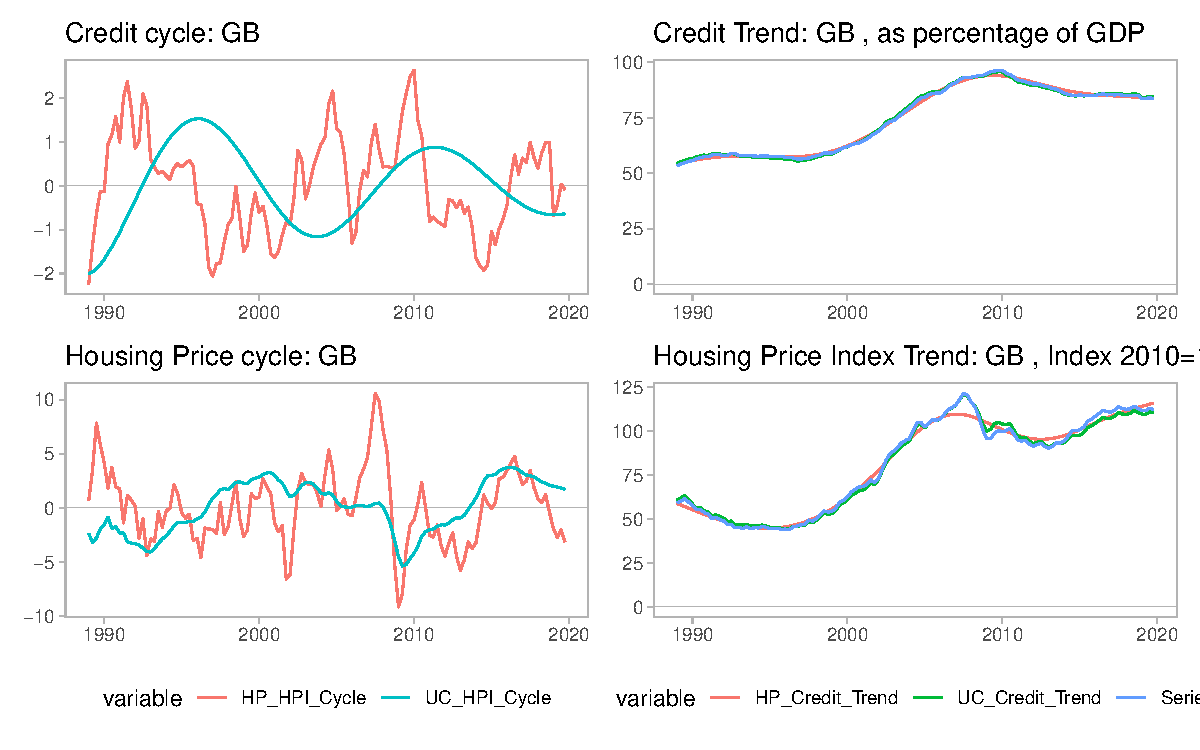
\includegraphics[width=0.85\linewidth]{../../Regression/VAR_2/Output/Graphs/HP_Credit_4graphs_GB} 

}

\caption{VAR(2) UK}\label{fig:unnamed-chunk-1}
\end{figure}

\begin{figure}

{\centering 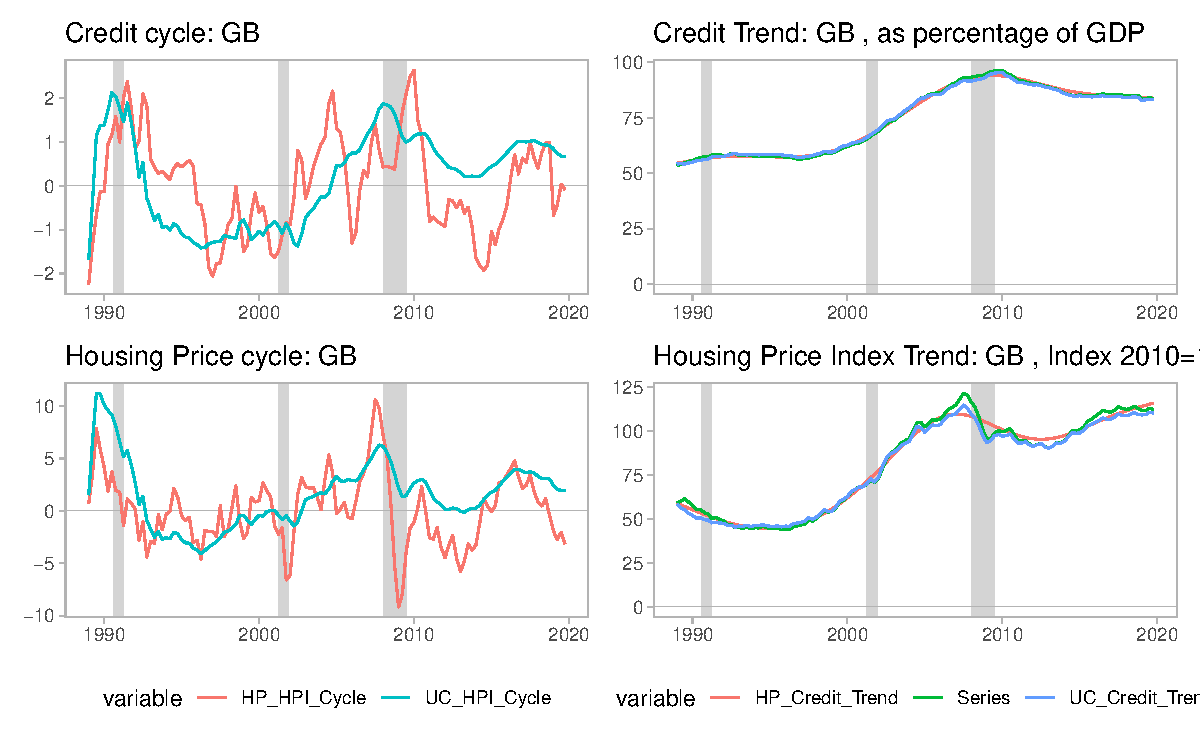
\includegraphics[width=0.85\linewidth]{../../Regression/VAR_2_crosscycle_1stlagonly/Output/Graphs/HP_Credit_4graphs_GB} 

}

\caption{VAR(2) Cross-cycle 1st lag only UK}\label{fig:unnamed-chunk-2}
\end{figure}

\begin{figure}

{\centering 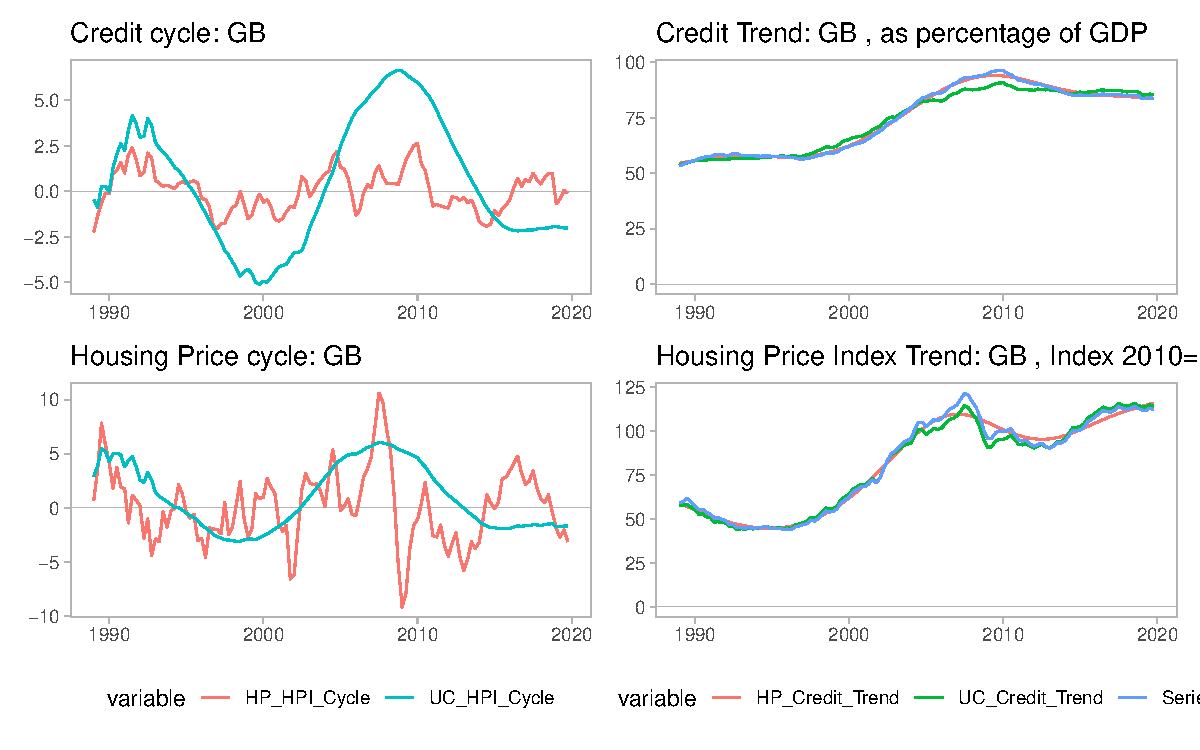
\includegraphics[width=0.85\linewidth]{../../Regression/VAR_2_crosscycle/Output/Graphs/HP_Credit_4graphs_GB} 

}

\caption{VAR(2) Cross-cycle 2 lags UK}\label{fig:unnamed-chunk-3}
\end{figure}

\begin{figure}

{\centering 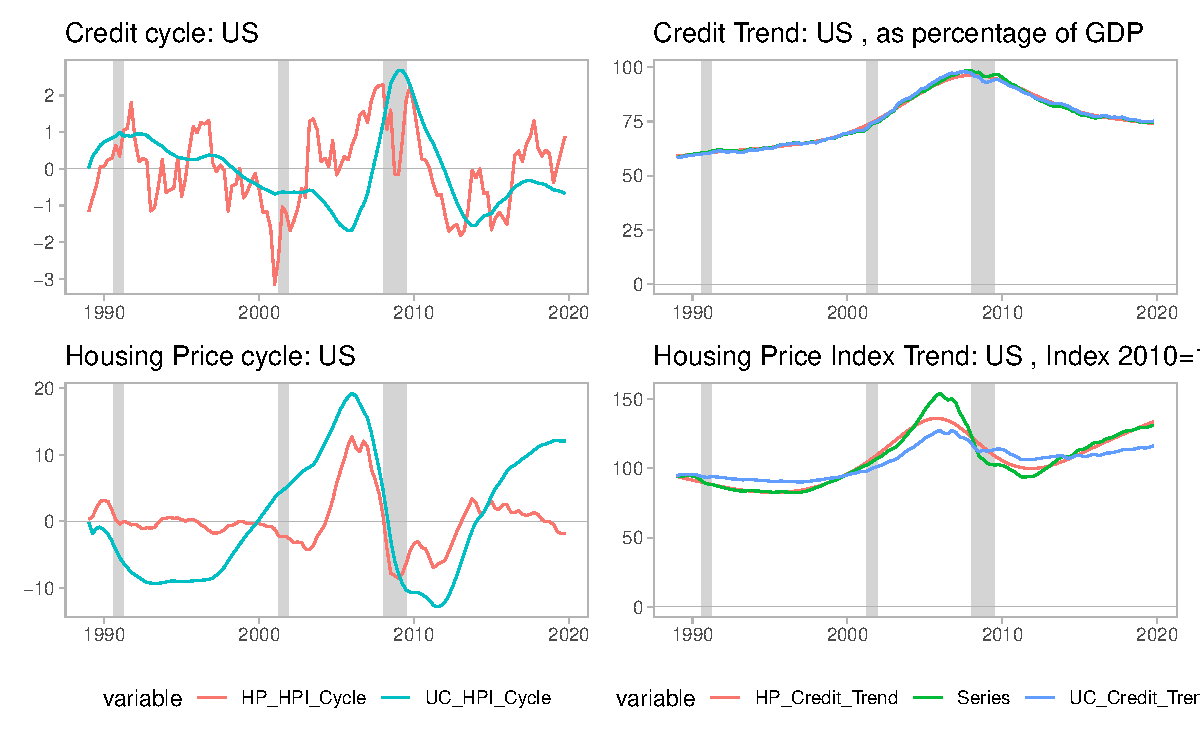
\includegraphics[width=0.85\linewidth]{../../Regression/VAR_2/Output/Graphs/HP_Credit_4graphs_US} 

}

\caption{VAR(2) US}\label{fig:unnamed-chunk-4}
\end{figure}

\begin{figure}

{\centering 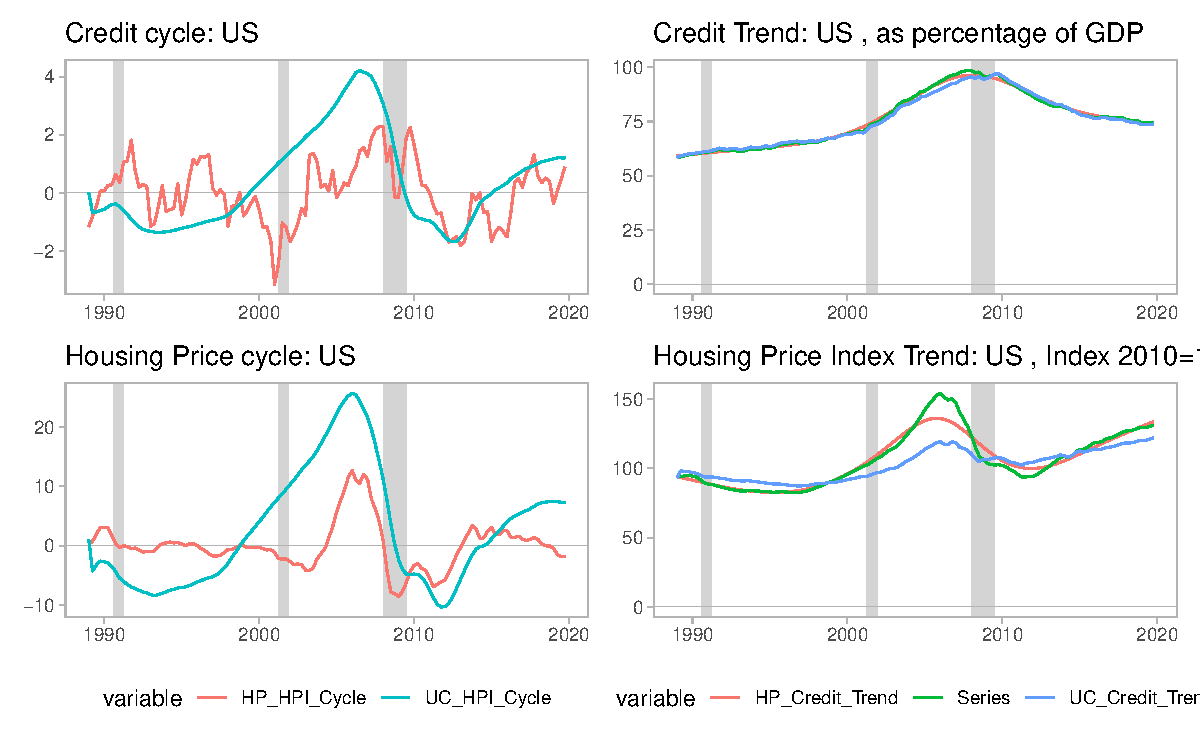
\includegraphics[width=0.85\linewidth]{../../Regression/VAR_2_crosscycle_1stlagonly/Output/Graphs/HP_Credit_4graphs_US} 

}

\caption{VAR(2) Cross-cycle 1st lag only US}\label{fig:unnamed-chunk-5}
\end{figure}

\begin{figure}

{\centering 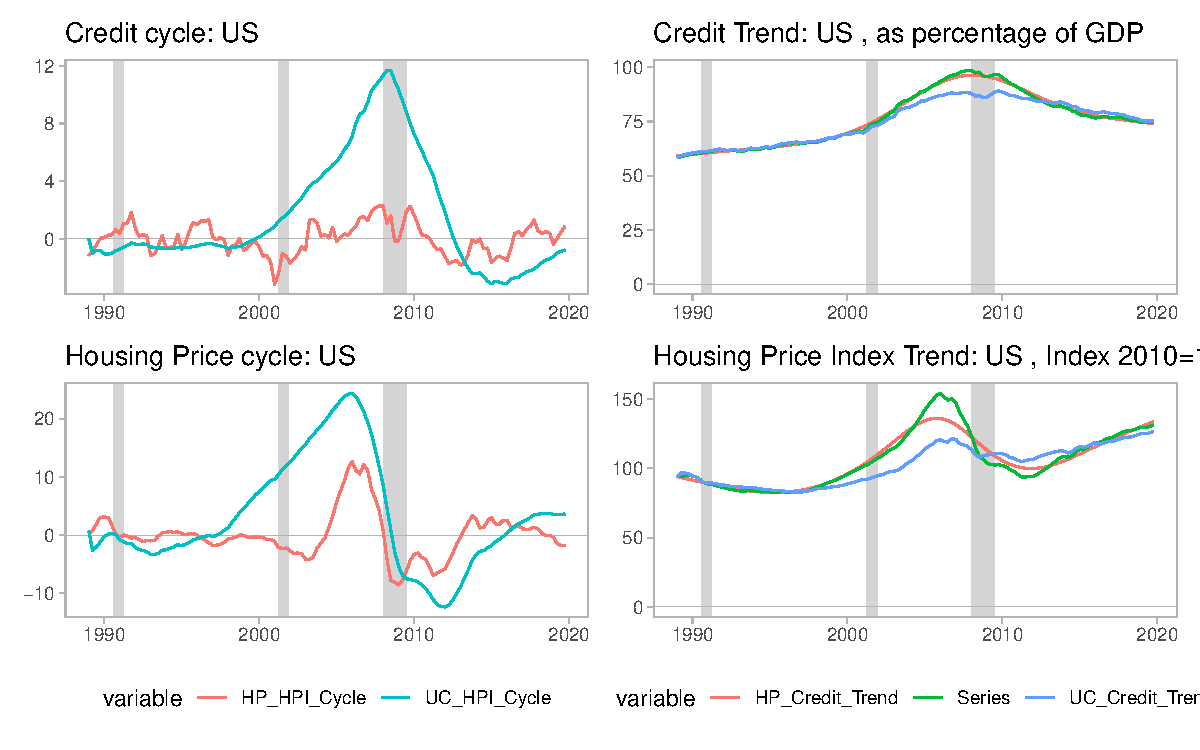
\includegraphics[width=0.85\linewidth]{../../Regression/VAR_2_crosscycle/Output/Graphs/HP_Credit_4graphs_US} 

}

\caption{VAR(2) Cross-cycle 2 lags}\label{fig:unnamed-chunk-6}
\end{figure}

        \pagebreak
        In this subsection, we decompose trend and cycle of household credit and housing price using the correlated unobserved component model. The stochastic trend in the multivariate UC model captures the long-run evolution in household credit, housing price, and the effect of the recent global financial crisis. In the long run, there is an increasing trend in the housing price index. The household credit trend is also increasing but since the series is credit to household as a ratio to GDP, the rate at which household credit trend increases is smaller than that of the housing price index. There is a downward movement of the trend components in both credit and housing price after the financial crisis. However, the housing price index trends made a quicker recovery than household credit did. 
        
        The cyclical components of the model capture the evolution of household credit, housing price, and their dynamic relationship. In Figures 1-6, we can see that there is an increase in credit transitory component before the financial crisis of 2008-2009 happened, and there is a negative shock to the transitory component of housing price after the recession is captured in the model as well.
        
        It is also important to point out that our models capture a significant bigger gap in transitory shock in both credit and house price than a Hodrick-Prescott (HP) filter would. This implies that when dealing with a time series of low frequency and long-term assets such as housing price, it is worthwhile to consider using the unobserved component model rather than simply applying an HP filter since it reveals more lower frequency information. The graphs indicate that the magnitude of transitory shocks the models capture is higher and the frequency of the movement of the cycles is lower than that of other methods (HP filter). The graphs also imply that the models detect a bigger credit gap in the UK (Figure 3), and also bigger gaps in household credit and house price in the US (Figure 4-6).     
        
        
        \subsection{Predictive ability of cyclical components}
        A novel contribution of this paper is to introduce the cross-cycle parameter $\phi^{xt}_h$ and $\phi^{xt}_{y}$ in which it measures the effect of a change in last periods' credit transitory component on the current housing price transitory component and vice versa. From Table 4 and 5, in both cross-cycle regressions in the UK and US, we can observe that there is a significant positive effect of last period credit cycle deviation on current housing cycle component ($\phi^{x1}_{h}$). While the coefficients of transitory housing index deviation on household credit ($\phi^{x1}_{y}$) are much smaller. This holds true for 2-crosscycle lags model also. This showed evidence that transitory shocks to household credit will cause a positive deviation in transitory housing price. However, transitory shocks to housing price have significantly smaller impact on household credit.
        

\hypertarget{robustness-check}{%
\section{ROBUSTNESS CHECK}\label{robustness-check}}

In this section, we check the robustness of our results by comparing the estimated trend-cycle from our approach with univariate trend-cycle decomposition using different methods. In addition to the estimation of the correlation between shocks to the permanent and transitory component, the use of multivariate model in theory should also provide us a superior measurement of trend and cycle components as compared to the univariate models. To test this hypothesis, we also perform trend-cycle decomposition using the univariate models (Figure \ref{fig:UKrobust} and \ref{fig:USrobust}). The univariate models include a HP filter model and a univariate VAR(2) UC model. The HP filter method uses an algorithm to smooth the original data series to estimate the trend component and the difference between them is the cyclical component. The parameter value \(\lambda\) is set at 1600 as suggested by Hodrick and Prescott for the quarterly data. The univariate UC model only uses the series of credit to household or house prices index to decompose a stochastic trend component and a cyclical component with the same specification as in the multivariate UC model.

\begin{figure}

{\centering 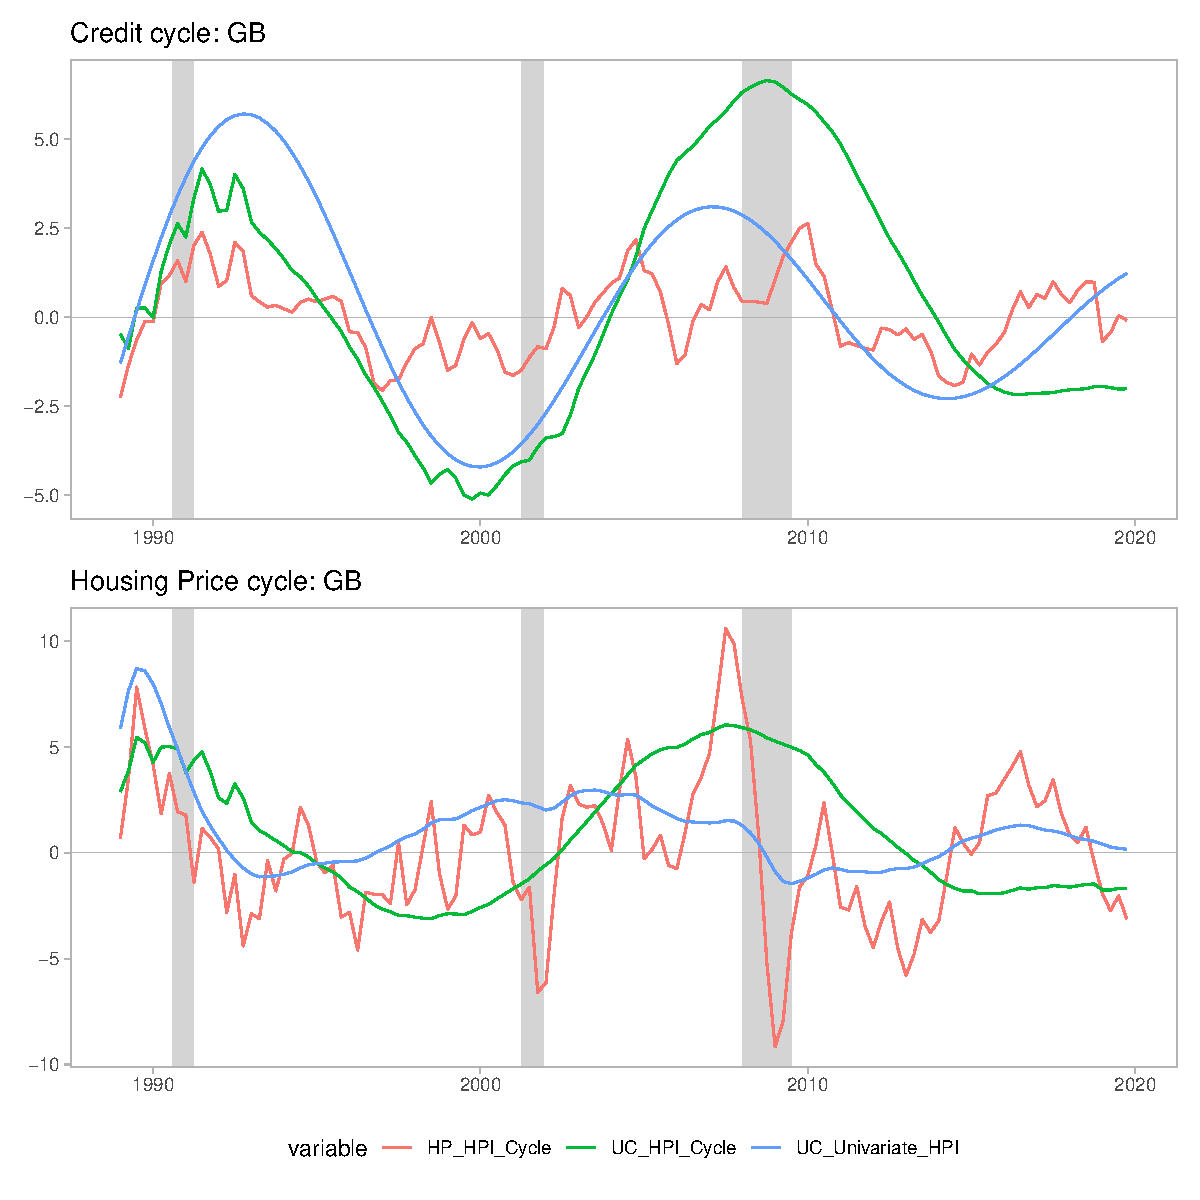
\includegraphics[width=0.85\linewidth]{../../Regression/AR_2/Output/graphs/HP_Credit_2graphs_GB} 

}

\caption{Comparing Multivariate UC cycles with alternate decompositions: UK}\label{fig:UKrobust}
\end{figure}

\begin{figure}

{\centering 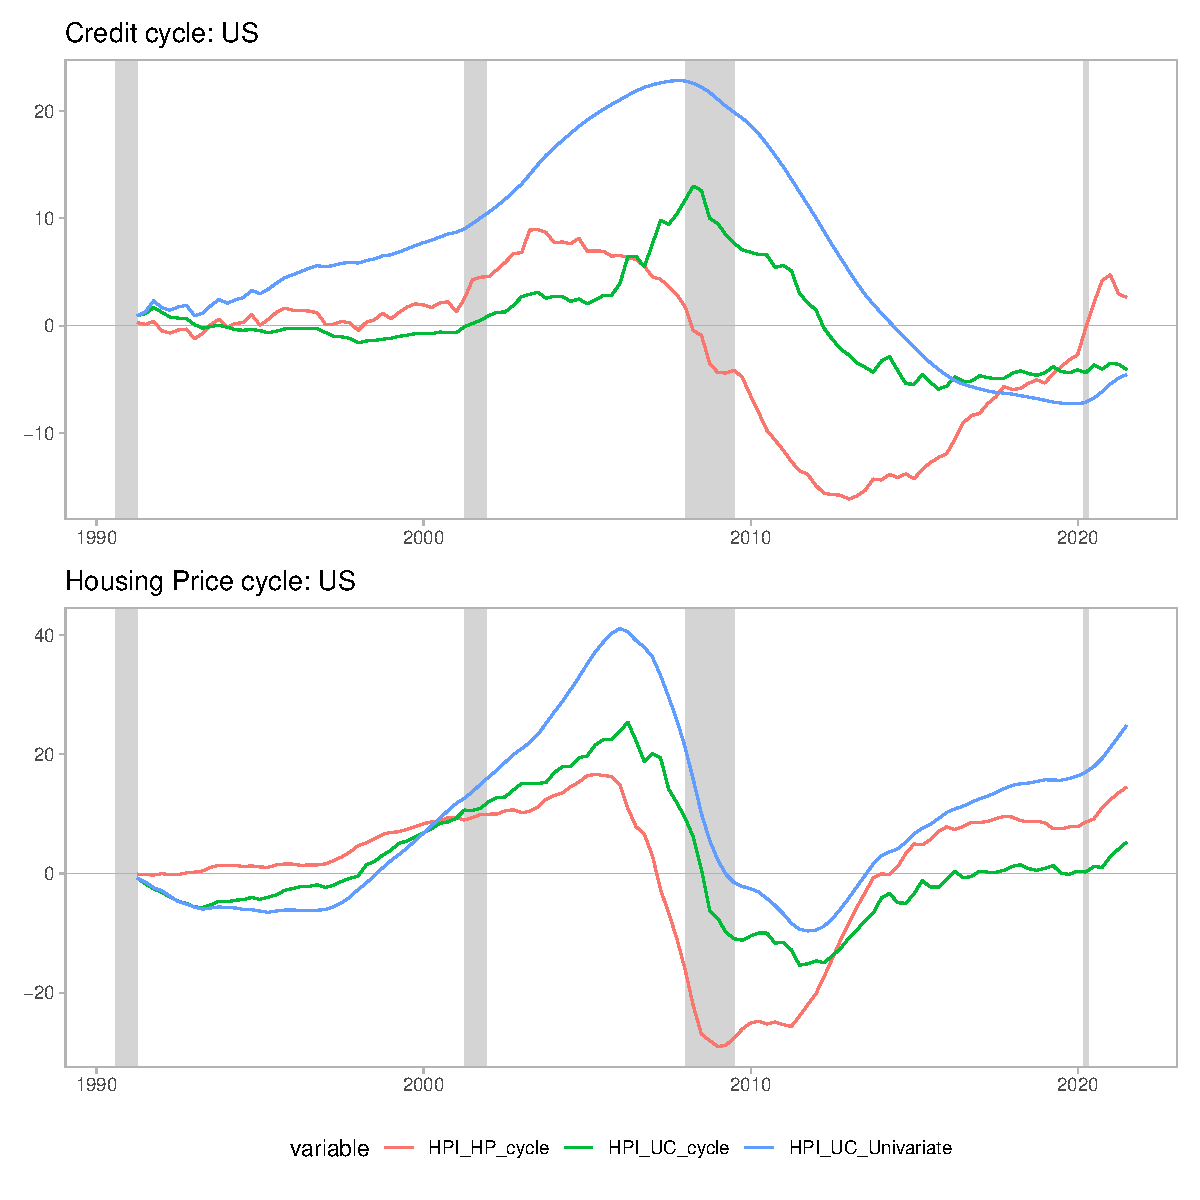
\includegraphics[width=0.85\linewidth]{../../Regression/AR_2/Output/graphs/HP_Credit_2graphs_US} 

}

\caption{Comparing Multivariate UC cycles with alternate decompositions: US}\label{fig:USrobust}
\end{figure}

\newpage

The results from Figure \ref{fig:UKrobust} and Figure \ref{fig:USrobust} suggest that the estimate of trend and cycles obtained from the multivariate UC model is capable of capturing the dynamics of the two variables during the sample period. The two univariate models, without assuming a linear trend, fail to generate realistic trend and cycle series by ignoring the relationship between the two variables of interest. The HP cycle seems to do very well at remaining stationary, but by doing so, it missed out in capturing the boom of house prices in the US leading to the Great Recession of 2009. The cycle from the univariate UC model, is close to the multivariate counter part but failed to fully indicate the magnitude of boom and bust in house prices in the UK before and after the crisis. Overall, it is clear from the analysis above that there is valuable pay-off in utilising information from extracting permanent and transitory components of credit to household and house prices index in order to study the dynamics of the two variables.

\hypertarget{conclusion}{%
\section{CONCLUSION}\label{conclusion}}

In this paper, we use a correlated multivariate unobserved component model to examine the hypothesis about the role of household credit on house prices and vice versa. In doing so, we decompose the movements of the two variables of interest into a permanent and transitory component. The correlations among the cyclical components support the idea that the rise of household credit is associated with a house prices above it long-run trend. Our multivariate model captures the dynamics features of the household credit and house prices series and performs better than univariate benchmarks in capturing the boom and bust during the last two decades. Additionally, employing cross correlation effects on the transitory components of the two series allows me to test the predictive ability of the cyclical components and found evidence to support that a household credit gap can positively predict a house prices gap. These findings suggests macroprudential policy implication since house prices are increasingly becoming a more important topic.

Further development for this paper should include studying on policy implication of credit and house price gaps with high magnitudes, introducing more robust optimal constraints on parameters to ensure stability rather than an ad-hoc approach of selecting weights. Additional examination of the multicollinearity and identification issues also need to be addressed.

\hypertarget{appendix}{%
\section*{APPENDIX}\label{appendix}}
\addcontentsline{toc}{section}{APPENDIX}

\hypertarget{model-estimation---priors-selection}{%
\subsection*{Model estimation - Priors selection}\label{model-estimation---priors-selection}}
\addcontentsline{toc}{subsection}{Model estimation - Priors selection}

The priors for autoregressive parameters in matrix F are taken from VAR regression of the HP filter cycle decomposition of the series.

For \(\beta_{0|0}\), I set \(\tau_{0|0}\) as the value HP filtered trend component and omit the first observation from the regression. \(c_{0|0}\) cycle components are also set to be equal to their HP filter counterpart. Variance \(var(\tau_{0|0}) =100+50*random\); while other measures of the starting covariance are set to be their unconditional values.

Starting standard deviation and correlation values are randomized within reasonable range.

\hypertarget{references}{%
\section*{References}\label{references}}
\addcontentsline{toc}{section}{References}

\hypertarget{refs}{}
\begin{CSLReferences}{1}{0}
\leavevmode\vadjust pre{\hypertarget{ref-agnello_economic_2018}{}}%
Agnello, L., Castro, V., \& Sousa, R. M. (2018). Economic {Activity}, {Credit Market Conditions}, and the {Housing Market}. \emph{Macroeconomic Dynamics}, \emph{22}, 1769--1789.

\leavevmode\vadjust pre{\hypertarget{ref-agnello_booms_2011}{}}%
Agnello, L., \& Schuknecht, L. (2011). Booms and busts in housing markets: {Determinants} and implications. \emph{Journal of Housing Economics}, \emph{20}, 171--190.

\leavevmode\vadjust pre{\hypertarget{ref-alessi_identifying_2018}{}}%
Alessi, L., \& Detken, C. (2018). Identifying excessive credit growth and leverage. \emph{Journal of Financial Stability}, \emph{35}, 215--225.

\leavevmode\vadjust pre{\hypertarget{ref-thaler_chapter_2005}{}}%
Barberis, N., Shleifer, A., \& Vishny, R. W. (2005). Chapter 12. {A Model} of {Investor Sentiment}. In R. H. Thaler (Ed.), \emph{Advances in {Behavioral Finance}, {Volume II}} (pp. 423--459). {Princeton University Press}.

\leavevmode\vadjust pre{\hypertarget{ref-bernanke_agency_1989}{}}%
Bernanke, B., \& Gertler, M. (1989). Agency {Costs}, {Net Worth}, and {Business Fluctuations}. \emph{American Economic Review}, 19.

\leavevmode\vadjust pre{\hypertarget{ref-beveridge_new_1981}{}}%
Beveridge, S., \& Nelson, C. R. (1981). A new approach to decomposition of economic time series into permanent and transitory components with particular attention to measurement of the {`business cycle.'} \emph{Journal of Monetary Economics}, \emph{7}, 151--174.

\leavevmode\vadjust pre{\hypertarget{ref-boissay_booms_2016}{}}%
Boissay, F., Collard, F., \& Smets, F. (2016). Booms and {Banking Crises}. \emph{Journal of Political Economy}, \emph{124}, 489--538.

\leavevmode\vadjust pre{\hypertarget{ref-bordalo_diagnostic_2018}{}}%
Bordalo, P., Gennaioli, N., \& Shleifer, A. (2018). Diagnostic {Expectations} and {Credit Cycles}. \emph{The Journal of Finance}, \emph{73}, 199--227.

\leavevmode\vadjust pre{\hypertarget{ref-burnside_understanding_2016}{}}%
Burnside, C., Eichenbaum, M., \& Rebelo, S. (2016). Understanding booms and busts in housing markets. \emph{Journal of Political Economy}, \emph{124}, 1088--1147.

\leavevmode\vadjust pre{\hypertarget{ref-capozza_anatomy_2004}{}}%
Capozza, D. R., Hendershott, P. H., \& Mack, C. (2004). An {Anatomy} of {Price Dynamics} in {Illiquid Markets}: {Analysis} and {Evidence} from {Local Housing Markets}. \emph{Real Estate Economics}, \emph{32}, 1--32.

\leavevmode\vadjust pre{\hypertarget{ref-davis_housing_2015}{}}%
Davis, M. A., \& Van Nieuwerburgh, S. (2015). Housing, {Finance}, and the {Macroeconomy}. In \emph{Handbook of {Regional} and {Urban Economics}} (Vol. 5, pp. 753--811). {Elsevier}.

\leavevmode\vadjust pre{\hypertarget{ref-di_maggio_credit-induced_2017}{}}%
Di Maggio, M., \& Kermani, A. (2017). Credit-{Induced Boom} and {Bust}. \emph{The Review of Financial Studies}, \emph{30}, 3711--3758.

\leavevmode\vadjust pre{\hypertarget{ref-durbin_time_2012}{}}%
Durbin, J., \& Koopman, S. J. (2012). \emph{Time series analysis by state space methods}. {Oxford university press}.

\leavevmode\vadjust pre{\hypertarget{ref-favara_credit_2015}{}}%
Favara, G., \& Imbs, J. (2015). Credit {Supply} and the {Price} of {Housing}. \emph{American Economic Review}, \emph{105}, 958--992.

\leavevmode\vadjust pre{\hypertarget{ref-favilukis_international_2012}{}}%
Favilukis, J., Kohn, D., Ludvigson, S., \& Van Nieuwerburgh, S. (2012). \emph{International {Capital Flows} and {House Prices}: {Theory} and {Evidence}} (No. w17751; p. w17751). {Cambridge, MA}: {National Bureau of Economic Research}.

\leavevmode\vadjust pre{\hypertarget{ref-favilukis_macroeconomic_2017}{}}%
Favilukis, J., Ludvigson, S. C., \& Van Nieuwerburgh, S. (2017). The {Macroeconomic Effects} of {Housing Wealth}, {Housing Finance}, and {Limited Risk Sharing} in {General Equilibrium}. \emph{Journal of Political Economy}, \emph{125}, 140--223.

\leavevmode\vadjust pre{\hypertarget{ref-geanakoplos_liquidity_2001}{}}%
Geanakoplos, J. (2001). \emph{Liquidity, {Default} and {Crashes}: {Endogenous Contracts} in {General Equilibrium}} (\{\{SSRN Scholarly Paper\}\} No. ID 284829). {Rochester, NY}: {Social Science Research Network}.

\leavevmode\vadjust pre{\hypertarget{ref-glaeser_housing_2008}{}}%
Glaeser, E. L., Gyourko, J., \& Saiz, A. (2008). Housing supply and housing bubbles. \emph{Journal of Urban Economics}, \emph{64}, 198--217.

\leavevmode\vadjust pre{\hypertarget{ref-glaeser_extrapolative_2017}{}}%
Glaeser, E. L., \& Nathanson, C. G. (2017). An extrapolative model of house price dynamics. \emph{Journal of Financial Economics}, \emph{126}, 147--170.

\leavevmode\vadjust pre{\hypertarget{ref-golosov_decentralized_2014}{}}%
Golosov, M., Lorenzoni, G., \& Tsyvinski, A. (2014). Decentralized {Trading With Private Information}. \emph{Econometrica}, \emph{82}, 1055--1091.

\leavevmode\vadjust pre{\hypertarget{ref-guerrieri_housing_2016}{}}%
Guerrieri, V., \& Uhlig, H. (2016). Housing and {Credit Markets}: {Bubbles} and {Crashes}. \emph{Handbook of Macroeconomics}, 110.

\leavevmode\vadjust pre{\hypertarget{ref-harrison_speculative_1978}{}}%
Harrison, J. M., \& Kreps, D. M. (1978). Speculative {Investor Behavior} in a {Stock Market} with {Heterogeneous Expectations}*. \emph{The Quarterly Journal of Economics}, \emph{92}, 323--336.

\leavevmode\vadjust pre{\hypertarget{ref-he_housing_2015}{}}%
He, C., Wright, R., \& Zhu, Y. (2015). Housing and liquidity. \emph{Review of Economic Dynamics}, \emph{18}, 435--455.

\leavevmode\vadjust pre{\hypertarget{ref-head_search_2014}{}}%
Head, A., Lloyd-Ellis, H., \& Sun, H. (2014). Search, {Liquidity}, and the {Dynamics} of {House Prices} and {Construction}. \emph{American Economic Review}, \emph{104}, 1172--1210.

\leavevmode\vadjust pre{\hypertarget{ref-hong_unified_1999}{}}%
Hong, H., \& Stein, J. C. (1999). A {Unified Theory} of {Underreaction}, {Momentum Trading}, and {Overreaction} in {Asset Markets}. \emph{The Journal of Finance}, \emph{54}, 2143--2184.

\leavevmode\vadjust pre{\hypertarget{ref-huang_rise_2019}{}}%
Huang, A., \& Kishor, N. K. (2019). The rise of dollar credit in emerging market economies and {US} monetary policy. \emph{The World Economy}, \emph{42}, 530--551.

\leavevmode\vadjust pre{\hypertarget{ref-huo_financial_2016}{}}%
Huo, Z., \& Ríos-Rull, J.-V. (2016). \emph{Financial {Frictions}, {Asset Prices}, and the {Great Recession}} {[}Preprint{]}. {Staff Report}.

\leavevmode\vadjust pre{\hypertarget{ref-jorda_betting_2015}{}}%
Jordà, Ò., Schularick, M., \& Taylor, A. M. (2015). Betting the house. \emph{Journal of International Economics}, \emph{96}, S2--S18.

\leavevmode\vadjust pre{\hypertarget{ref-jorda_great_2016}{}}%
Jordà, Ò., Schularick, M., \& Taylor, A. M. (2016). The great mortgaging: Housing finance, crises and business cycles. \emph{Economic Policy}, \emph{31}, 107--152.

\leavevmode\vadjust pre{\hypertarget{ref-jorda_macrofinancial_2017}{}}%
Jordà, Ò., Schularick, M., \& Taylor, A. M. (2017). Macrofinancial {History} and the {New Business Cycle Facts}. \emph{NBER Macroeconomics Annual}, \emph{31}, 213--263.

\leavevmode\vadjust pre{\hypertarget{ref-justiniano_credit_2019}{}}%
Justiniano, A., Primiceri, G. E., \& Tambalotti, A. (2019). Credit supply and the housing boom. \emph{Journal of Political Economy}, \emph{127}, 1317--1350.

\leavevmode\vadjust pre{\hypertarget{ref-kermani_cheap_2012}{}}%
Kermani, A. (2012). Cheap credit, collateral and the boom-bust cycle. \emph{University of California-Berkeley, Working Paper}.

\leavevmode\vadjust pre{\hypertarget{ref-kim_state-space_1999}{}}%
Kim, C.-J., \& Nelson, C. R. (1999). State-space models with regime switching: Classical and {Gibbs}-sampling approaches with applications. \emph{MIT Press Books}, \emph{1}.

\leavevmode\vadjust pre{\hypertarget{ref-kishor_forecasting_2020}{}}%
Kishor, N. K. (2020). Forecasting real-time economic activity using house prices and credit conditions. \emph{Journal of Forecasting}.

\leavevmode\vadjust pre{\hypertarget{ref-kishor_time_2015}{}}%
Kishor, N. K., Kumari, S., \& Song, S. (2015). Time variation in the relative importance of permanent and transitory components in the {U}.{S}. Housing market. \emph{Finance Research Letters}, \emph{12}, 92--99.

\leavevmode\vadjust pre{\hypertarget{ref-kiyotaki_credit_1997}{}}%
Kiyotaki, N., \& Moore, J. (1997). Credit {Cycles}. \emph{Journal of Political Economy}, \emph{105}, 211--248.

\leavevmode\vadjust pre{\hypertarget{ref-kiyotaki_money_1989}{}}%
Kiyotaki, N., \& Wright, R. (1989). On {Money} as a {Medium} of {Exchange}. \emph{Journal of Political Economy}, \emph{97}, 927--954.

\leavevmode\vadjust pre{\hypertarget{ref-knoll_return_2016}{}}%
Knoll, K. (2016). \emph{Return predictability in international housing markets, 1870-2014} (PhD thesis). Dissertation draft, University of Bonn.

\leavevmode\vadjust pre{\hypertarget{ref-knoll_no_2017}{}}%
Knoll, Katharina, Schularick, M., \& Steger, T. (2017). No {Price Like Home}: {Global House Prices}, 1870-2012. \emph{American Economic Review}, \emph{107}, 331--353.

\leavevmode\vadjust pre{\hypertarget{ref-martin_theoretical_2010}{}}%
Martin, A., \& Ventura, J. (2010). \emph{Theoretical {Notes} on {Bubbles} and the {Current Crisis}} (Working \{\{Paper\}\} No. 16399). {National Bureau of Economic Research}.

\leavevmode\vadjust pre{\hypertarget{ref-mian_house_2011}{}}%
Mian, A., \& Sufi, A. (2011). House {Prices}, {Home Equity}-{Based Borrowing}, and the {US Household Leverage Crisis}. \emph{American Economic Review}, \emph{101}, 2132--2156.

\leavevmode\vadjust pre{\hypertarget{ref-mian_credit_2018}{}}%
Mian, A., \& Sufi, A. (2018). \emph{Credit {Supply} and {Housing Speculation}} (No. w24823). {National Bureau of Economic Research}.

\leavevmode\vadjust pre{\hypertarget{ref-morley_slow_2007}{}}%
Morley, J. C. (2007). The {Slow Adjustment} of {Aggregate Consumption} to {Permanent Income}. \emph{Journal of Money, Credit and Banking}, \emph{39}, 615--638.

\leavevmode\vadjust pre{\hypertarget{ref-myerson_model_2012}{}}%
Myerson, R. B. (2012). A {Model} of {Moral}-{Hazard Credit Cycles}. \emph{Journal of Political Economy}, \emph{120}, 847--878.

\leavevmode\vadjust pre{\hypertarget{ref-ortalo-magne_housing_2006}{}}%
Ortalo-Magne, F., \& Rady, S. (2006). Housing market dynamics: {On} the contribution of income shocks and credit constraints. \emph{The Review of Economic Studies}, \emph{73}, 459--485.

\leavevmode\vadjust pre{\hypertarget{ref-samuelson_exact_1958}{}}%
Samuelson, P. A. (1958). An {Exact Consumption}-{Loan Model} of {Interest} with or without the {Social Contrivance} of {Money}. \emph{Journal of Political Economy}, \emph{66}, 467--482.

\leavevmode\vadjust pre{\hypertarget{ref-scheinkman_overconfidence_2003}{}}%
Scheinkman, J. A., \& Xiong, W. (2003). Overconfidence and {Speculative Bubbles}. \emph{Journal of Political Economy}, \emph{111}, 1183--1220.

\leavevmode\vadjust pre{\hypertarget{ref-schularick_credit_2012}{}}%
Schularick, M., \& Taylor, A. M. (2012). Credit {Booms Gone Bust}: {Monetary Policy}, {Leverage Cycles}, and {Financial Crises}, 1870-2008. \emph{American Economic Review}, \emph{102}, 1029--1061.

\leavevmode\vadjust pre{\hypertarget{ref-simsek_belief_2013}{}}%
Simsek, A. (2013). Belief {Disagreements} and {Collateral Constraints}. \emph{Econometrica}, \emph{81}, 1--53.

\leavevmode\vadjust pre{\hypertarget{ref-stein_prices_1995}{}}%
Stein, J. C. (1995). Prices and {Trading Volume} in the {Housing Market}: {A Model} with {Down}-{Payment Effects}*. \emph{The Quarterly Journal of Economics}, \emph{110}, 379--406.

\leavevmode\vadjust pre{\hypertarget{ref-wright_buyers_2014}{}}%
Wright, R., \& Wong, Y.-Y. (2014). Buyers, {Sellers}, and {Middlemen}: {Variations} on {Search}-{Theoretic Themes}. \emph{International Economic Review}, \emph{55}, 375--397.

\end{CSLReferences}

\end{document}
